
\documentclass[12pt,a4paper, twoside, openright]{article}
\usepackage{graphicx}
\usepackage                              {subfigure}
\usepackage     [utf8]                  {inputenc}
\usepackage     [T1]                    {fontenc}
\usepackage                             {color}
\usepackage                             {amsmath}
\usepackage							   {amssymb}
\usepackage     [ngerman]               {babel}
\usepackage                             {cite}
\usepackage                             {hyperref}
\usepackage                             {multirow}
\usepackage  							{epstopdf}
\usepackage		[onehalfspacing]			{setspace}
\usepackage[left=2.5cm,right=2.5cm,top=2.5cm,bottom=2cm]{geometry}

\usepackage{listings}

\usepackage{etoolbox}
\pretocmd\section{\cleardoublepage}{}%
  {\errmessage{Patching \noexpand\section failed}}

\begin{document}
%Silbentrennung (funktioniert auf deutsch nicht immer)
\hyphenation{ar-bei-ten}
\hyphenation{Ar-beits-punkt Ar-beits-punk-te Ar-beits-punk-ten}
\hyphenation{Auf-l"o-sung Auf-l"o-sun-gen}
\hyphenation{aus-schlie"s-lich}
\hyphenation{Aus-tausch-teil-chen}
\hyphenation{Be-schrei-bung}
\hyphenation{Be-stim-mung}
\hyphenation{Bo-son Bo-son-en}
\hyphenation{brei-tet}
\hyphenation{De-tek-tor-ma-ter-ial}
\hyphenation{Dis-kri-mi-na-tor Dis-kri-mi-na-tors}
\hyphenation{ein-ge-zeich-net}
\hyphenation{End-zu-stand}
\hyphenation{Ent-falt-ungs-me-tho-de}
\hyphenation{ent-spre-chen-den}
\hyphenation{Ent-wick-lung-en}
\hyphenation{Er-eig-nis Er-eig-nisse}
\hyphenation{ge-ring}
\hyphenation{Kop-plungs-konst-an-te}
\hyphenation{Mes-sun-gen}
\hyphenation{Miss-iden-ti-fi-ka-tions-ra-te}
\hyphenation{Mo-dell Mo-del-le}
\hyphenation{m"uss-ten}
\hyphenation{or-tho-go-nal}
\hyphenation{pa-ra-me-tri-siert}
\hyphenation{re-gu-la-ri-sie-ren re-gu-la-ri-sier-ten}
\hyphenation{Schwer-punkts-en-er-gie Schwer-punkts-en-er-gien}
\hyphenation{sei-ner}
\hyphenation{selbst}
\hyphenation{si-mu-liert-en si-mu-liert si-mu-lier-en si-mu-lierte}
\hyphenation{Sym-me-trie-grup-pe}
\hyphenation{sys-te-ma-tisch-en}
\hyphenation{Ty-pi-scher-wei-se ty-pi-scher-wei-se}
\hyphenation{um-fang-reich um-fang-rei-cher}
\hyphenation{Un-si-cher-heit Un-si-cher-hei-ten}
\hyphenation{Un-ter-grund Un-ter-grund-er-eig-nis-se Un-ter-grund-er-eig-nis-sen}
\hyphenation{ver-an-schau-licht}
\hyphenation{Wahr-schein-lich-keit}
\hyphenation{Wechsel-wirk-ung Wechsel-wir-kun-gen}
\hyphenation{wei-cher}
\hyphenation{Wei-te-ren}
\hyphenation{wes-halb}
\hyphenation{Wir-kungs-quer-schnitts Wir-kungs-quer-schnitt}
\hyphenation{zwi-schen}
\hyphenation{Kennt-nisse}
\hyphenation{konn-ten}

\title{Studium von Top-Quark-Paaren am LHC   \vspace{2cm}  \\ \centerline{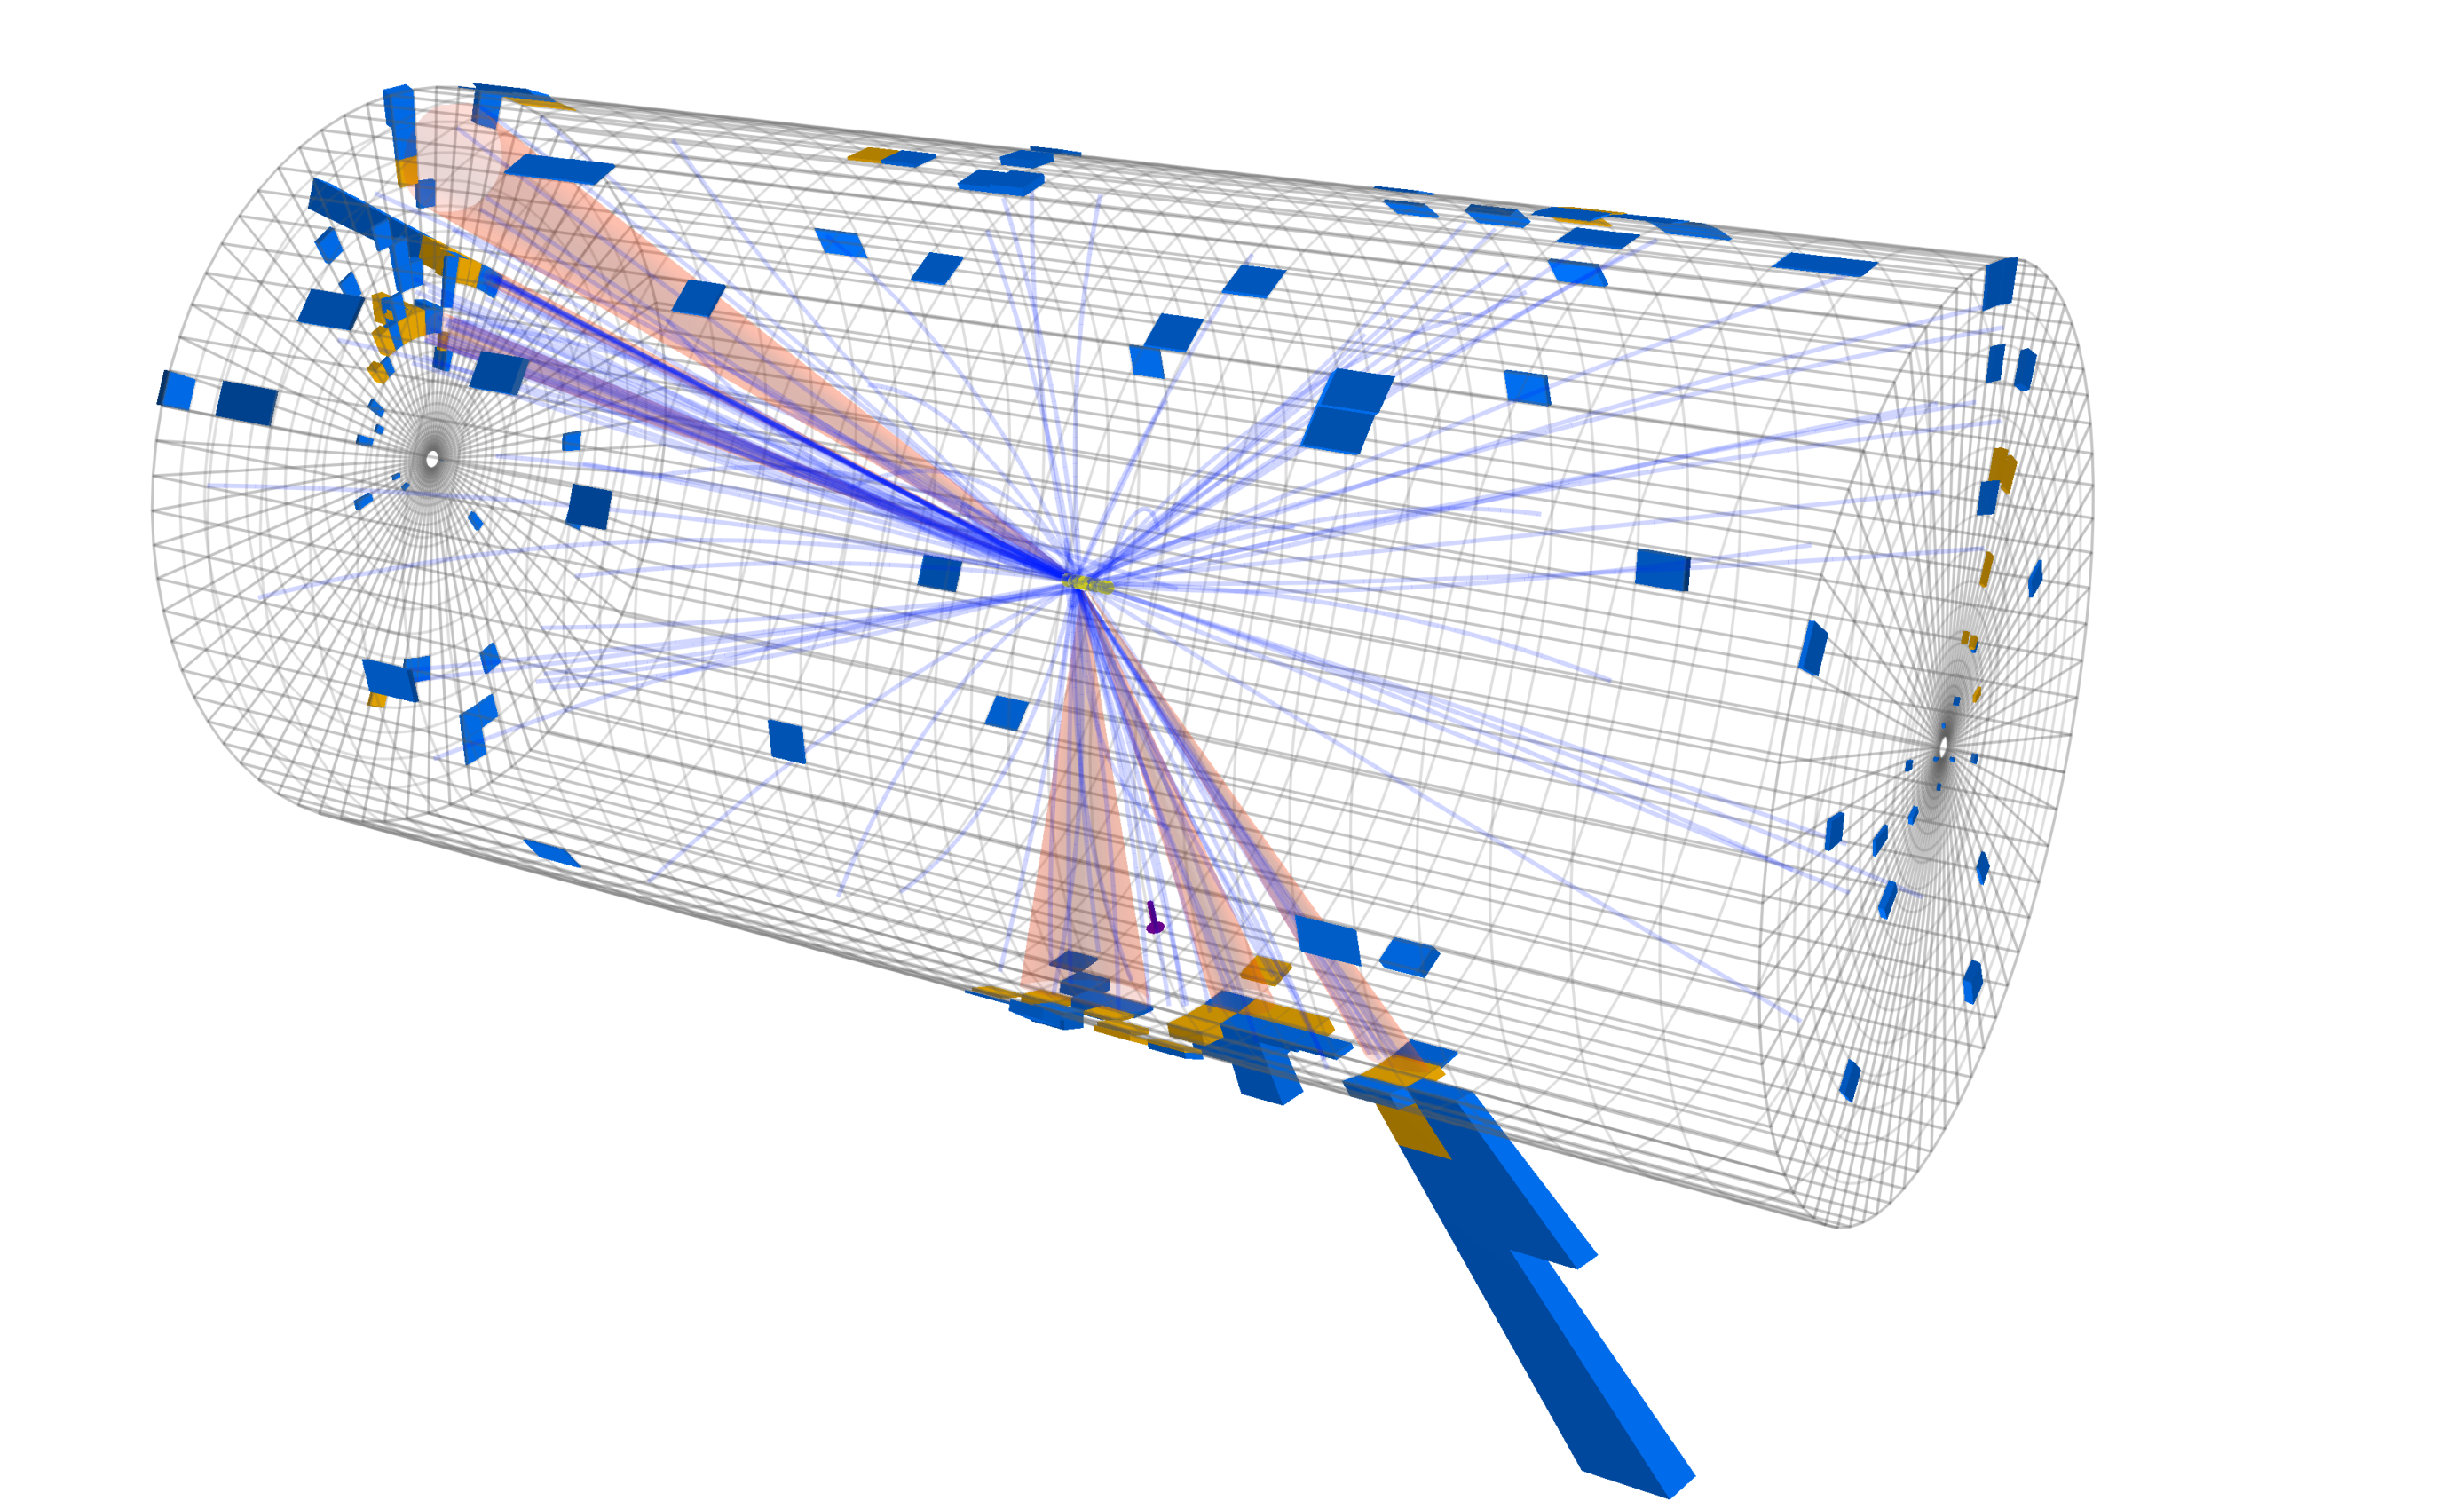
\includegraphics[scale=0.22]{eventdisplay.png}} \vspace{2cm}} 
\date{2018}
\author{Jens Multhaup, Arne Reimers, Marc St\"over \\ Univsersit\"at Hamburg \\ Praktikum f\"ur Fortgeschrittene}
\maketitle
\thispagestyle{empty}
\newpage \thispagestyle{empty}
\tableofcontents
\thispagestyle{empty}
\newpage\thispagestyle{empty}
\cleardoublepage{}



\section{Einleitung}
\label{intro}
Es ist das Ziel der Elementarteilchenphysik, die elementaren Bausteine der Natur sowie die fundamentalen Gesetze ihrer Wechselwirkung zu entdecken und zu untersuchen.
 Man glaubt heute, dass die uns bekannte Materie aus einigen wenigen Sorten von Teilchen zusammengesetzt ist, zwischen denen als elementar angesehene Kr\"afte herrschen.
 Um in diese Welt der kleinsten Strukturen einzudringen, werden hohe Teilchenenergien ben\"otigt. Der zur Zeit gr\"o\ss{} te und leistungsf\"ahigste Teilchenbeschleuniger den die
 Menschheit je gebaut hat, ist der LHC. Hier werden Protonen zur Kollision gebracht, um die Eigenschaften der elementaren Teilchen genau zu studieren oder v\"ollig neue 
 Teilchen zu entdecken. Am LHC stehen daf\"ur bislang unerreichte Energien zur Verfuegung, was nie gekannte Pr\"azision bei der Vermessung des massereichsten bekannten Teilchens,
 des Top-Quarks, erm\"oglicht. 

Sie werden bei diesem Versuch eine Messung mit realen Daten, die bei einer Schwerpunktsenergie von 7\,TeV vom CMS Detektor aufgenommen wurden, durchf\"uhren.
 Sie sollen selbstst\"andig den Produktionswirkungsquerschnitt von Top-Quark-Paaren ermitteln und auch die Top-Quark-Masse rekonstruieren.
 Dabei wenden Sie aktuelle Methoden der experimentellen Teilchenphysik an und lernen die gr\"undliche Behandlung von statistischen und systematischen Unsicherheiten.
 Am Ende k\"onnen sie Ihr Ergebnis mit offiziell am LHC gemessenen Werten vergleichen!

%Mit diesem Versuch vermitteln wir Ihnen einen Eindruck des Arbeitsalltages eines experimentellen Teilchenphysikers. Folgende Bereiche der Physik m\"ochten wir Ihnen dabei vermitteln
%\begin{itemize}
%	\item Elementarteilchen und ihre Wechselwirkungen (mit Materie)
%	\item Teilchendetektoren- und Identifikation
%	\item (Top-Quark-)Physik an Proton-Proton-Collidern bei hohen Schwerpunktsenergien
%\end{itemize}
	Eine Messung an Collider-Experimenten besteht im Allgemeinen aus mehreren Komponenten. Die Zerfallsprodukte eines Kanals werden von dem Detektor gemessen, sodass anschlie\ss{}end Techniken ben\"otigt werden um die Zerfallsobjekte der richtigen Zerfallskaskade zuzuordnen. In diesem Versuch wenden wir uns dem Zerfall von Top-Quark-Paaren zu, wie schematisch in Abbildung \ref{ttbarsemilep} dargestellt. Ihre Aufgabe wird es sein, diesen Zerfallsbaum mit Hilfe einer Analyse-Software zu rekonstruieren und von anderen Standard-Modell-Prozessen zu unterscheiden.
\begin{figure}[h]
\centerline{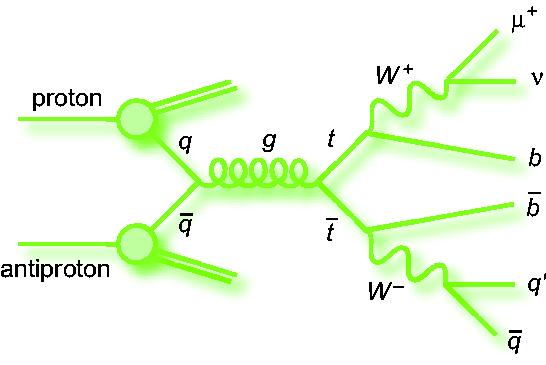
\includegraphics[scale=0.5]{pics_feynman_ttbar_mujets}}
\caption{Feynman-Diagramm eines Top-Antitop-Zerfalls. Im Endzustand sind zwei Quarks, zwei b-Quarks, ein Myon sowie ein Neutrino.}
\label{ttbarsemilep}
\end{figure}

F\"ur die Versuchsdurchf\"uhrung stellen wir Ihnen einen Unix-Rechner und ein Analyse-Framework zur Verf\"ugung. Dieses Framework ist selbstverst\"andlich noch sehr
 unvollst\"andig und wird w\"ahrend der Versuchsdurchf\"uhrung von Ihnen vervollst\''andigt und erweitert. Kenntnisse in der Programmiersprache C\texttt{++} sind von Vorteil, 
werden aber nicht vorausgesetzt. Bearbeiten Sie das kurze Tutorial auf
%TODO
\url{https://www.desy.de/~reimersa/Public/Teaching/LHCTop/Cplusplus.pdf}, um sich mit der Syntax in C\texttt{++} vertraut zu machen.\\



\section{Theoretische Grundlagen}
\label{sm_chapter}
In diesem Kapitel wollen wir Ihnen den theoretischen Hintergrund, der f"ur diesen Versuch relevant ist, vermitteln. Dazu fassen wir die relevantesten Aspekte des Standardmodells (SM) der Teilchenphysik,
das die fundamentalen Bestandteile und Wechselwirkungen der Natur beschreibt, in Abschnitt \ref{kapsm} zusammen.
Eine detaillierte Einf\"uhrung finden Sie in der entsprechenden Fachliteratur \cite{Griffiths, Berger}. Da das Top-Quark in diesem Versuch eine besondere Rolle spielt,
wird es in Abschnitt \ref{kaptop} noch einmal gesondert eingef\"uhrt und diskutiert.

% +++++++++++ Standardmodell und Top-Quark +++++++++++++++++
\subsection{Das Standardmodell der Teilchenphysik}
\label{kapsm}
Das Standardmodell der Teilchenphysik bildet den wichtigsten theoretischen Rahmen f\"ur die Ph\"anomene der Teilchenphysik und der gro\ss{}e Erfolg des Modells ist beeindruckend.
So wurden viele Vorhersagen des Standardmodells durch zahlreiche Experimente sehr genau best\"atigt. Insbesondere die Entdeckung vorhergesagter Elementarteilchen verdeutlicht dessen M\"achtigkeit.
Und dennoch deckt das SM in seiner jetzigen Form nicht alle Beobachtungen ab. So ist unter anderem die Gra\-vi\-ta\-tion nicht im SM enthalten. Des Weiteren gibt es Hinweise auf dunkle Materie und dunkle Energie, die weder direkt durch ein Experiment beobachtet werden konnten, noch durch das SM vorhergesagt sind.
\\
\\
Nach heutigem Wissensstand setzt sich die gesamte sichtbare Materie unseres Universums aus den fundamentalen Teilchen des Standardmodells zusammen.
Diese unterteilt man nach ihrem Spin in Fermionen (Spin-$1/2$) und Bosonen (Spin-$1$).\\
Innerhalb der Fermionen unterscheidet man zwischen geladenen ($Q = -1$) und neutralen ($Q = 0$) Leptonen, sowie up-artige ($Q = 2/3$) und down-artige ($Q = -1/3$) Quarks.
Abschlie\ss{}end werden die verschiedenen Leptonen und Quarks jeweils nach aufsteigender Masse in Paaren zusammengefasst und bilden die drei Generationen der Elementarteilchen. 
Zus\"atzlich dazu enth\"alt das Standardmodell zu jedem Teilchen ein Antiteilchen mit den selben Eigenschaften, aber umgekehrter Ladung.
Eine Auflistung der Fermionen ist in Tabelle \ref{Fermionen} zu finden.\\
% Tabelle: Fermionen
\begin{table}[bp]
\centering
\begin{tabular}{c|c||ccc}
  \cline{3-5}
   \multicolumn{2}{c|}{\multirow{2}{*}{}} & \multicolumn{3}{c}{Generationen}\\
   \multicolumn{2}{c|}{} & 1. & 2. & 3. \\
  \hline
  \multirow{2}{*}{{Leptonen}} & Neutral ($Q=0$) & $\nu_{e}$ & $\nu_{\mu}$ & $\nu_{\tau}$ \\
   \cline{2-5}
   & Geladen ($Q=-1$) & $e$ & $\mu$ & $\tau$ \\
  \hline \hline
  \multirow{2}{*}{{Quarks}} & up-artig ($Q=+\frac{2}{3}$) & $u$ & $c$ & $t$ \\
  \cline{2-5}
   & down-artig ($Q=-\frac{1}{3}$) & $d$ & $s$ & $b$ \\
  \hline
\end{tabular}
	  	\caption{Fermionen des SM mit ihrer Ladung (Q)~\cite{pdg}. }
	  		\label{Fermionen}
\end{table}
\\
\\
Die Wechselwirkungen zwischen den Teilchen werden durch die Eichbosonen vermittelt. Dazu geh\"oren das Photon ($\gamma$), die geladenen W-Bosonen ($W^{\pm}$), das neutrale $Z^{0}$-Boson, sowie die 8 Gluonen.
Eine \"Ubersicht der Bosonen und deren Eigenschaften findet sich in Tabelle \ref{Eichbosonen}. \\
\\
Die elektromagnetische Wechselwirkung wird durch den Austausch virtueller Photonen vermittelt. Photonen koppeln zu Teilchen mit elektrischer Ladung, sind jedoch selbst elektrisch neutral und k\"onnen
folglich nicht mit sich selbst wechselwirken. Die zugrundeliegende Theorie ist die Quantenelektrodynamik (QED), die auf der $U(1)_{Q}$-Sym\-me\-trie\-grup\-pe basiert.\\
\\
Die schwache Wechselwirkung wird \"uber die $W^{\pm}$- und $Z^{0}$-Bosonen \"ubertragen. Diese vermitteln zwischen den Fermionen mit schwachem Isospin $T_{3}$. 
Durch die hohen Massen der W-Bosonen von $m_{W} = 80,4\,\mathrm{GeV/c^{2}}$ und der Z-Masse von $m_{Z} = 91,2\,\mathrm{GeV/c^{2}}$ ist die Reichweite der Wechselwirkung sehr gering.
Im Bestreben die Kr\"afte des Standardmodells zu Vereinheitlichen gelang es die elektromagnetische und schwache Wechselwirkung miteinander zu verkn\"upfen.
Es resultiert die elektroschwache Theorie, die auf der $SU(2)_{L}\times SU(1)_{Y}$-Symmetrie beruht. Die Quantenzahl $Y = 2(Q - T_{3})$ ist dabei die Hyperladung.\\
Ein wichtiges Ph\"anomen der elektroschwachen Wechselwirkung ist die M\"oglichkeit der Quarks durch Kopplung an ein W-Boson nicht nur in ein Quark der selben Generation, 
sondern auch anderer Generationen \"uberzugehen. Jedes Quark tr\"agt eine sogenannte \textit{Flavour}-Quantenzahl mit sich, weshalb man auch von Flavour-\"andernden geladenen Str\"omen spricht. 
Die \"Ubergangswahrscheinlichkeit eines Quark-Flavours zu einem anderen wird \"uber die Ca\-bibbo-\-Ko\-ba\-ya\-shi-\-Maska\-wa\-(CKM)-\-Matrix beschrieben, die wie folgt lautet \cite{pdg}:
\begin{equation}
\textbf{V}_{CKM}=\begin{pmatrix} V_{ud} & V_{us} & V_{ub} \\ V_{cd} & V_{cs} & V_{cb} \\ V_{td} & V_{ts} & V_{tb} \end{pmatrix}=\begin{pmatrix} 0,974 & 0,225 & 0,004 \\ 0,225 & 0,973 & 0,041 \\ 0,009 & 0,040 & 0,999 \end{pmatrix}
\label{CKMmatrix}
\end{equation}
\\
F\"ur geladenen Leptonen wurde bisher kein solcher \"Ubertritt der Generationen beobachtet. Jedoch konnte in den letzten Jahren mit Hilfe verschiedener gro\ss{}er Neutrino-Experimente die Neutrinooszillation 
nachgewiesen werden. Der oszillierende \"Ubergang der Neutrinos in den drei Generationen ist der entscheidende Hinweis darauf, dass Neutrinos eine Masse besitzen.\\
\\
Masselose Gluonen stellen die Austauschteilchen der starken Wechselwirkung dar. Sie koppeln an die \textit{Farbladung}, die in den Zust\"anden blau, rot und gr\"un sowie den entsprechenden Anti-Zust\"anden auftreten.
Die zugrundeliegende Theorie ist die Quantenchromodynamik (QCD) mit ihrer Symmetriegruppe $SU(3)_{C}$\footnote{$C$ steht f\"ur \textit{colour} und meint in diesen Zusammenhang die Farbzust\"ande der 
starken Wechselwirkung.}. Aus der Gruppe der Leptonen tragen lediglich Quarks Farbladung. Dar\"uber hinaus tr\"agt das Gluon selbst Farbladung mit sich, sodass eine Selbstwechselwirkung unter Gluonen
m\"oglich ist. Können somit bei hohen Energien und damit kleinen Abst\"anden der Quarks und Gluonen noch als quasi-freie Teilchen behandelt werden, ist dies mit anwachsendem Abschand nicht mehr möglich.
Kommt es in Folge einer Teilchenkollision zur Separierung von Quarks und Gluonen wächst der einzige freie Parameter ($\alpha_{s}$) und die Energie des Farbfeldes stetig an. 
Sie steigt solange an, bis es energetisch g\"unstiger ist ein neues Quark-Antiquark Paar zu bilden. Dies wiederholt sich so lange, bis die Energie des Feldes nicht mehr ausreicht um ein neues Paar zu bilden.
Diesen Prozess bezeichnet man als Hadronisierung und den entstehenden kollimierten Teilchenschauer als Jet. 
\\
\begin{table}[tp]
\centering
\begin{tabular}{c||c|c|c}
Eichboson & Masse\,[GeV] & Wechselwirkung & Materieteilchen \\ \hline\hline
8 Gluonen & 0 & stark & Quarks \\ \hline
\multirow{2}{*}{$W^{\pm}$- und $Z^{0}$-Bosonen} & $m_{W}=80,4$ & schwach, & \multirow{2}{*}{Quarks, Leptonen} \\
 & $m_{Z}=91,2$ & elektromagnetisch & \\ \hline
Photon & 0 & elektromagnetisch & Quarks, geladene Leptonen\\ \hline
\end{tabular}
	  	\caption{Die Eichbosonen des SM mit ihren Massen, Wechselwirkungen und den Materie\-teilchen, an die sie koppeln.}
	  		\label{Eichbosonen}
\end{table}


% ======================
% ++++++Top Quark+++++++
% ======================
\subsection{Physik des Top-Quarks}
\label{kaptop}
Seit seiner Entdeckung im Jahr 1995 am Proton-Antiproton-Beschleuniger Tevatron, spielt das Top-Quark eine bedeutende Rolle in der Teilchenphysik. Das liegt insbesondere daran,
dass es mit einer Masse von $m_{t}=173,34\pm 0,76$\,GeV \cite{ATLAS:2014wva} das Schwerste aller Quarks ist.\\
W\"ahrend am Tevatron Top-Quarks bei einer Schwerpunkts\-energie von $\sqrt{s}=1,96$\,TeV\footnote{Bei der Entdeckung des Top-Quarks entsprach die Schwerpunkts\-energie am Tevatron $\sqrt{s}=1,8$\,TeV.
Erst 2001 wurde die Schwerpunkts\-energie auf 1,96\,TeV erh"oht.} erzeugt wurden, ist seit 2010 eine Produktion bei 7\,TeV bzw. 8\,TeV durch den Large Hadron Collider (LHC) m\"oglich.
Bereits 2011 wurden über 800\,000 Top-Quark-Paare am LHC erzeugt, was die M\"oglichkeit offenbart, die Eigenschaften des Top-Quarks sehr pr\"azise zu untersuchen. Dar\"uber hinaus erm\"oglicht es zahlreiche Suchen nach neuer Physik jenseits des Standardmodells, bei der Top-Quarks eine wichtige Rolle spielen.\\
Im Folgenden geht es um die Erzeugung von Top-Quark-Paaren, sowie um deren Zerfall -- vorrangig unter den Vorraussetzungen des LHC -- und dar\"uber hinaus um das Top-Quark jenseits des SM. Ein umfangreicher \"Uberblick zur Physik des Top-Quarks kann in \cite{Bernreuther, Schilling} gefunden werden.


% ======================
% +++ttbar Produktion+++
% ======================
\subsubsection{Top-Quark-Produktion am LHC}
%\footnotetext{\textbf{I}nitial \textbf{S}tate \textbf{R}adiation: Abstrahlung eines Teilchens im Anfangszustand. Die Abstrahlung eines Teilchens im Endzustand wird entsprechend als \textbf{F}inal \textbf{S}tate \textbf{R}adiation bezeichnet.}
\begin{figure}[t]
	\centering
	\includegraphics[scale=0.80]{Theorie/toppairfeynman.eps}
	\caption[Feynman-Diagramme zur $t\overline{t}$-Produktion in verschiedenen Kan"alen]{Feynman-Diagramme zur $t\overline{t}$-Produktion in verschiedenen Kan"alen. In den ersten beiden Reihen wird die $t\overline{t}$-Produktion in f"uhrender Ordnung gezeigt. In der dritten Reihe ist, aufgrund der ISR bzw. $g$-Schleife, die $t\overline{t}$-Produktion in der n"achst-f"uhrenden Ordnung zu sehen.}
	\label{toppairproduction}
\end{figure}
\begin{figure}[t!]
	\centering
	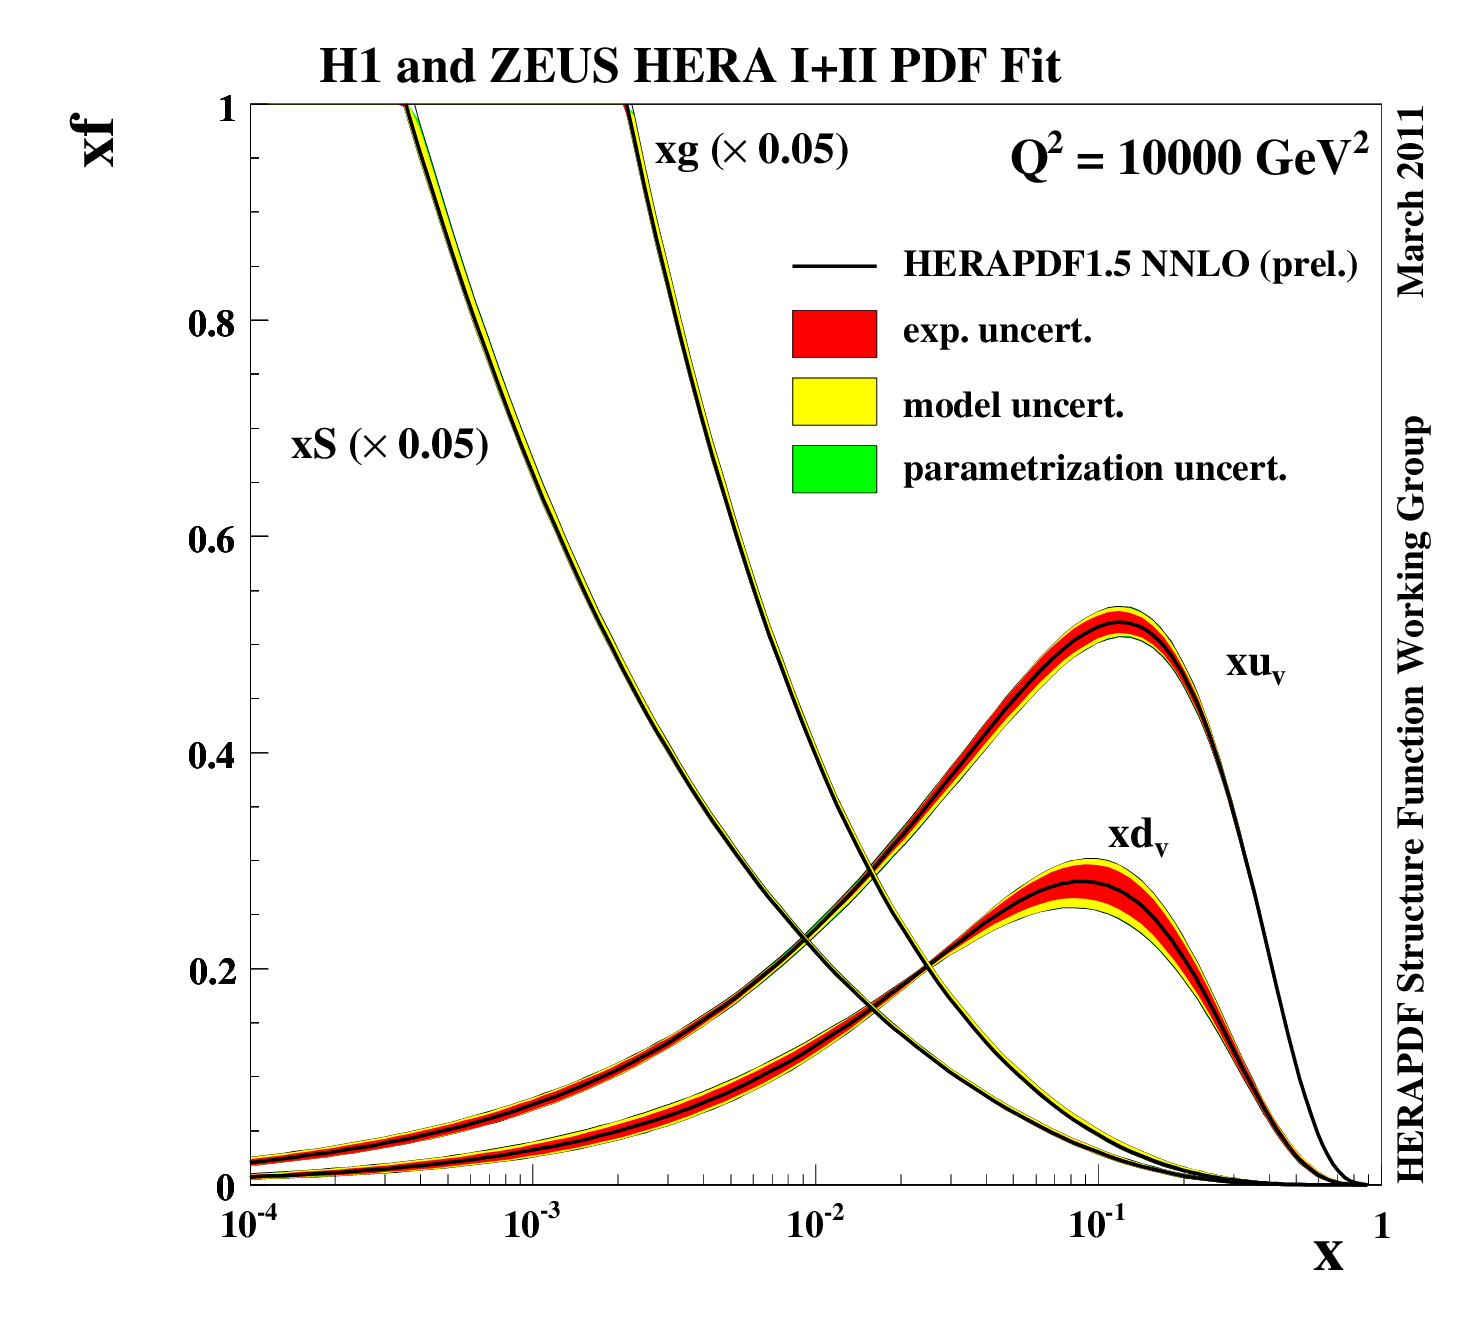
\includegraphics[scale=0.30]{Theorie/herapdf2.png}
	\caption[Parton-Dichte-Funktionen (PDFs) des Protons als Funktion des Impulsbruchteils $x$]{Parton-Dichte-Funktionen (PDFs) des Protons als Funktion des Impulsbruchteils $x$. F"ur einen Viererimpuls"ubertrag von $Q^{2}=10000$\,GeV$^{2}$ sind die PDFs der Valenzquarks ($u_{v},d_{v}$), Seequarks (S) und Gluonen (g) abgebildet \cite{combinedhera}.}
	\label{herannlo}
\end{figure}
Die Produktion von Top-Quark-Paaren im SM wird haupts\"achlich \"uber die starke Wechselwirkung vermittelt. Top-Quark-Paare k\"onnen sowohl in Quark-Antiquark-Annihilationen als auch in Gluon-Gluon-Fusionen produziert werden. Abbildung \ref{toppairproduction} veranschaulicht diese Prozesse. Zur Erzeugung eines $t\overline{t}$-Paares muss die Schwerpunkts\-energie der wechselwirkenden Partonen $\hat{s}$ mindestens der doppelten Top-Quark-Masse ($\approx$350\,GeV) entsprechen. Aus diesem Grund m\"ussen Partonen, unter der Annahme von $x_{1}=x_{2}$, den Impulsbruchteil
\begin{equation}
x_{1,2}\geq \frac{350\,\text{GeV}}{1,96\,\text{TeV}}\approx 0,2 \text{ (Tevatron)},\,\,x_{1,2}\geq \frac{350\,\text{GeV}}{8\,\text{TeV}}\approx 0,04 \text{ (LHC)}
\end{equation}
besitzen, um $t\overline{t}$-Paare erzeugen zu k\"onnen. Abbildung \ref{herannlo} ist zu entnehmen, dass die Valenz\-quarks bei einem Impulsbruchteil von 0,2 in den PDFs dominant sind. Deshalb \"uberwiegt die Quark-Antiquark-Annihilation zur $t\overline{t}$-Paar-Produktion am Tevatron zu ei\-nem Anteil von ungef"ahr 85\,\%. Am LHC liegt ein \"ahnlicher Anteil zugunsten der Gluon-Gluon-Fusion vor. Die dortige Schwerpunkts\-energie von 8\,TeV erlaubt zur $t\overline{t}$-Produktion kleinere Impulsbruchteile, bei denen die Gluondichten steil ansteigen.
\\
\\
Am LHC wird bei einer Schwerpunkts\-energie $\sqrt{s}=8$\,TeV ein inklusiver $t\overline{t}$-Wirkungs\-querschnitt von $229_{-26}^{+24}$\,pb in NLO \cite{Cacciari:2011hy} und $246_{-11}^{+9}$\,pb in NNLO vorhergesagt \cite{Czakon:2013goa}. In Abbildung \ref{ttprodcross} ist der $t\overline{t}$-Produktionswirkungsquerschnitt in gen"aherter NNLO-Pr"azision eingezeichnet. Die Messwerte bei $\sqrt{s}=1,96$\,TeV mit dem D0- und CDF-Experiment sowie bei $\sqrt{s}=7$\,TeV und $\sqrt{s}=8$\,TeV mit dem CMS-Experiment stimmen gut mit der Vorhersage "uberein.\\
\\
%F"ur die Beschreibung der $t\overline{t}$-Signalereignisse werden in dieser Arbeit die Monte-Carlo-Ereignisgeneratoren \Powheg und \Madgraph verwendet. In der Generierung der Ereignisse liegen zwischen \Powheg und \Madgraph dadurch Unterschiede vor, dass Matrixelemente, Teilchenschauer, Hadronisations- oder Pile-Up-Effekte verschieden berechnet werden. So berechnet beispielsweise \Powheg 2$\rightarrow$2 Matrixelemente in NLO, w"ahrend von \Madgraph 2$\rightarrow$n Prozesse simuliert werden k"onnen, wobei $n\leq 9$ ist. \\ \\
Zus\"atzlich zu der $t\overline{t}$-Produktion k\"onnen \"uber die schwache Wechselwirkung einzelne Top-Quarks erzeugt werden. Die Produktionskan\"ale in niedrigster Ordnung sind Abbildung \ref{singletopprod}
zu entnehmen. Der $t$-Kanal, bei dem das Top-Quark \"uber die Fusion eines $W$-Bosons und eines $b$-Quarks erzeugt wird, ist dabei der dominante Prozess.
Der inklusive Wirkungsquerschnitt des $t$-Kanals betr\"agt 87,2\,pb am LHC bei einer Schwerpunktsenergie von 8\,TeV. Da $u$-Quarks die dominanten Valenzquarks in den PDFs bei $pp$-Beschleunigern sind,
ist die Top-Quark-Produktion im $t$-Kanal ladungsasymmetrisch. Es hat des Weiteren zur Folge, dass die Produktion von Top-Quarks (56,4\,pb) der Produktion von Antitop-Quarks (30,7\,pb) mit einem Verh\"altnis
von ungef\"ahr 2:1 \"uberwiegt. Im $s$-Kanal liegt mit dem Zerfall in ein Top und ein Antibottom (3,79\,pb) und deren Antiteilchen (1,76\,pb) der analoge Sachverhalt vor.\\
\\
Die assoziierte Produktion ($tW$-Kanal) einzelner Top-Quarks ist ladungssymmetrisch, weil im Anfangszustand ein Gluon und ein (Anti)b-Quark enthalten ist. F\"ur beide Zust\"ande betr\"agt der vorhergesagte Wirkungsquerschnitt 11,1\,pb \cite{Kidonakis:1449411}.

\begin{figure}[ht]
	\centering
	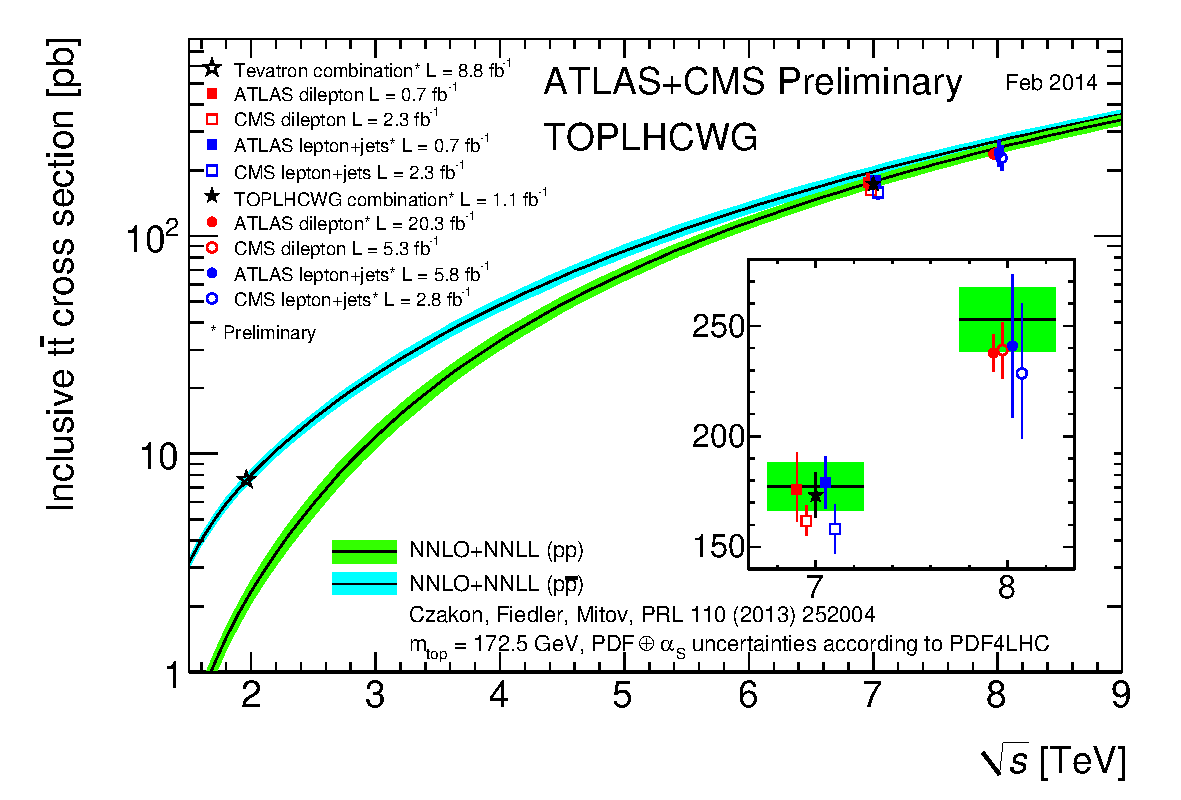
\includegraphics[scale=0.70]{Theorie/ttproductioncrosssection_new.pdf}
	\caption[Der $t\overline{t}$-Produktionswirkungsquerschnitt in Abh\"angigkeit der Schwer\-punkts\-energie]{Der $t\overline{t}$-Produktionswirkungsquerschnitt in Abh\"angigkeit der Schwer\-punkts\-energie. Eingezeichnet sind die Messungen am Tevatron bei $\sqrt{s}=1,96$\,TeV, sowie die Messungen des CMS- und ATLAS-Experiments am LHC bei 7\,TeV und 8\,TeV in verschiedenen Zerfallskan\"alen \cite{prodcrosssectionatlascms}.}
	\label{ttprodcross}
\end{figure}

\begin{figure}[ht]
	\centering
	\includegraphics[scale=0.80]{Theorie/singletopfeynman.eps}
	\caption[Feynman-Diagramme zur Produktion einzelner Top-Quarks in f\"uhrender Ordnung]{Feynman-Diagramme zur Produktion einzelner Top-Quarks in f\"uhrender Ordnung.}
	\label{singletopprod}
\end{figure}



%++++++++++++++++++++++++++++++++++++++++++++++++++++++++
%\footcite{textbf{I}nitial \textbf{S}tate \textbf{R}adiation: Abstrahlung eines Partons im Anfangszustand. Bei Abstrahlungen im Endzustand spricht man entsprechend von textbf{F}inal \textbf{S}tate \textbf{R}adiation}

\subsubsection{Masse und Zerfall des Top-Quarks}
\label{massanddecaytop}
Die Polmasse des Top-Quarks ist ein fundamentaler Parameter des SM. Direkte Messungen am Tevatron ergeben einen Wert von $m_{t}=173,2\pm 0,9$\,GeV \cite{Lancaster:2011wr}. Mit einer Unsicherheit von 0,5\,\% ist die Top-Quark-Masse damit sehr pr\"azise vermessen.
\\
\\
Das Top-Quark kann im SM ausschlie\ss{}lich in ein down-artiges Quark und ein $W$-Boson zerfallen. Die jeweilige Zerfallsrate ist proportional zum Quadrat der Elemente der CKM-Matrix $|V_{tq}|^{2}$ ($q=d,s,b$), sodass der Zerfall in ein W-Boson und ein $b$-Quark mit ca. 99,9\% dominiert (vgl. Gleichung (\ref{CKMmatrix})). Die totale Zerfallsbreite $\Gamma_{t}$ des Top-Quarks im SM ist $\Gamma_{t}=1,33\,\text{GeV} $ \cite{Jezabek:1988iv}. Die gro\ss{}e Zerfallsbreite des Top-Quarks hat eine sehr kurze Lebensdauer von $\tau_{t}=\frac{1}{\Gamma_{t}}\approx 5\cdot 10^{-25}$\,s zur Folge. Die Zeitskala, die Quarks zur Hadronisierung ben\"otigen, liegt in der Gr\"o\ss{}enordnung $\tau_{\text{had}}\sim 10^{-24}$\,s. Top-Quarks zerfallen demzufolge bevor sie hadronisieren k\"onnen, sodass keine gebundenen $t\overline{t}$-Zust\"ande (\textit{Toponium}) existieren.\\
\\
Entsprechend des Zerfalls eines Top-Quarks hat der Zerfall eines $t\overline{t}$-Paares, $t\overline{t}\rightarrow b\overline{b}W^{+}W^{-}$, zwei W-Bosonen und b-Quarks im Endzustand. Die W-Bosonen zerfallen anschlie\ss{}end entweder in ein geladenes Lepton und das zugeh\"orige Neutrino oder in ein $q\overline{q}$-Paar. Der Zerfall in Quark-Paare, die Top-Quarks enthalten, ist aus kinematschen Gr\"unden verboten, da die Masse des Top-Quarks die Masse des W-Bosons \"ubersteigt. Der Zerfall des W-Bosons l\"asst somit drei Zerfallskan\"ale f\"ur den $t\overline{t}$-Zerfall zu, die in Abbildung \ref{leadingorderttbar} dargestellt sind. Die Verzweigungsverh\"altnisse der $t\overline{t}$-Zerfallskan\"ale sind in Tabelle \ref{TopZerfallsraten} zu finden.  \\
\begin{figure}[ht]
	\centering
	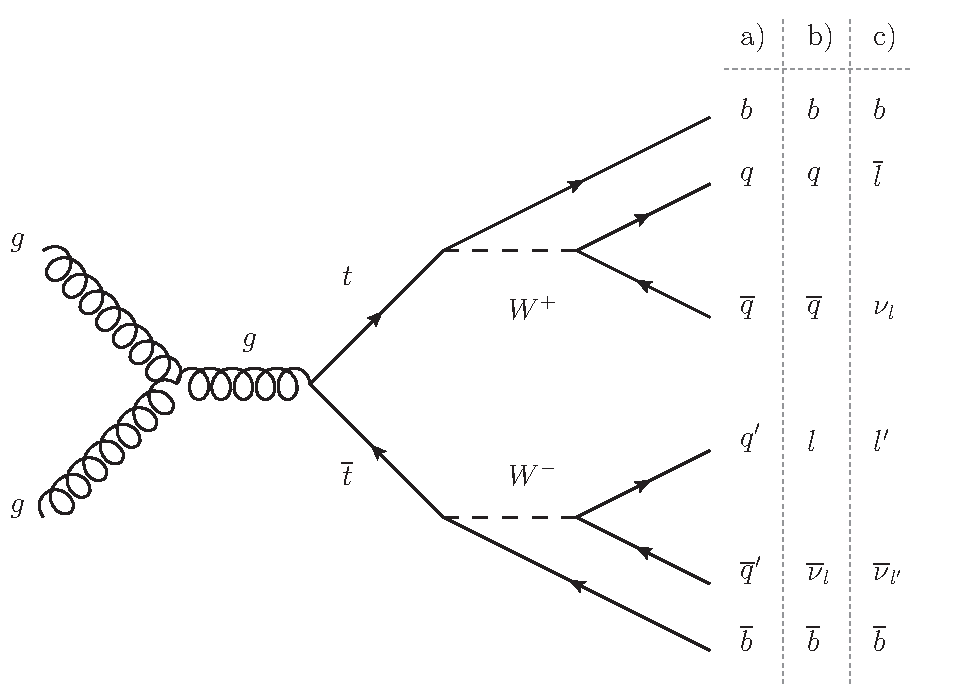
\includegraphics[scale=0.80]{Theorie/leadingorderttproduction-eps-converted-to}
	\caption[Feynman-Diagramm zur $t\overline{t}$-Produktion in f"uhrender Ordnung durch $gg$-Fusion]{Feynman-Diagramm zur $t\overline{t}$-Produktion in f\"uhrender Ordnung durch $gg$-Fusion. Gezeigt ist au"sserdem der weitere Zerfall im voll hadronischen\,(a)), semi\-lep\-tonischen\,(b)) und dileptonischen\,(c)) Kanal.}
	\label{leadingorderttbar}
\end{figure}

\subsubsection*{Voll hadronischer Kanal}
Die gr\"o\ss{}te Zerfallsrate mit 45,7\,\% liegt vor, wenn beide $W$-Bosonen hadronisch zerfallen:
\begin{equation*}
t\overline{t}\rightarrow b\overline{b}W^{+}W^{-}\rightarrow b\overline{b}q\overline{q}'q''\overline{q}'''
\end{equation*}
Neben der gro\ss{}en Zerfallsrate hat dieser Kanal den Vorteil, dass alle Teilchen im Endzustand (zumindest prinzipiell) gemessen werden k\"onnen. Dem entgegen steht ein sehr gro\ss{}er hadronischer Untergrund, der die Rekonstruktion von Quarks zum entsprechenden $t\overline{t}$-Ereignis erschwert.

\subsubsection*{Semileptonischer Kanal}

Die zweitgr\"o\ss{}te Rate (43,8\,\%) f\"ur einen Endzustand liegt vor, wenn eines der $W$-Bosonen hadronisch und das andere leptonisch zerf\"allt:
\begin{equation*}
t\overline{t}\rightarrow b\overline{b}W^{+}W^{-}\rightarrow b\overline{b}q\overline{q}'l\overline{\nu}_{l}
\end{equation*}
In der Praxis wird der semileptonische Kanal auf ein Elektron oder Myon im Endzustand beschr\"ankt, weil das $\tau$-Lepton weiter in Neutrinos und Hadronen bzw. Myonen und Elektronen zerf\"allt, ehe es detektiert werden kann\footnote{Prozesse, bei denen das $\tau$-Lepton in ein Myon oder Elektron zerf\"allt werden jedoch mit ber\"ucksichtigt.}. Die Zerfallsrate f\"ur diesen Kanal reduziert sich damit auf 29,8\,\%. Dessen ungeachtet vereint der semileptonische Zerfalls\-kanal die Vorteile einer gro\ss{}en Zerfallsrate und eines \"uberschaubaren Untergrundes. Die Hauptuntergrundquellen sind W- und Z-Bosonen in Verbindung mit Jets (sogenannte \textit{W-} bzw. \textit{Z-Jets}), einzelne Top-Quarks sowie QCD-Ereignisse. Des Weiteren wird die Rekonstruktion eines $t\overline{t}$-Ereignisses dadurch erschwert, dass das Neutrino nicht detektiert wird. \\
F\"ur diesen Praktikumsversuch wird der semileptonische $t\overline{t}$-Zerfallskanal mit einem My\-on (Myon+ Jets-Kanal) im Endzustand betrachtet.

\subsubsection*{Dileptonischer Kanal}
Der dileptonische Zerfallskanal hat mit 10,5\,\% die kleinste Zerfallsrate. Beide $W$-Bosonen zerfallen leptonisch, sodass zwei verschieden geladene Leptonen sowie zwei Neutrinos im Endzustand vorliegen:
\begin{equation*}
t\overline{t}\rightarrow b\overline{b}W^{+}W^{-}\rightarrow l\overline{\nu}_{l}\overline{l}'\nu_{l'}
\end{equation*}
Da die geladenen Leptonen verh\"altnism\"a\ss{}ig leicht vom Untergrund unterschieden werden k\"onnen, hat der dileptonische Zerfallskanal die reinste Signatur. Aufgrund der fehlenden Energie der beiden Neutrinos jedoch, kann die Struktur des $t\overline{t}$-Ereignisses nur sehr schwer rekonstruiert werden. Des Weiteren besteht die bereits f\"ur den semileptonischen Zerfalls\-kanal beschriebene Problematik, dass es sich bei einem geladenen Lepton oder beiden geladenen Leptonen um ein $\tau$-Lepton bzw. zwei $\tau$-Leptonen handelt. Schlie\ss{}t man $\tau$-Leptonen im Endzustand aus, reduziert sich die Zerfallsrate auf 4,6\,\%.


\begin{table}[ht]
\centering
\begin{tabular}{lc|lc}
Kanal & Rate\,[\%] & Kanal & Rate\,[\%] \\ \hline\hline
Dileptonisch & 10,50 $\pm$ 0,12 & $ee$ & 1,16 $\pm$ 0,02 \\
 &  & $\mu\mu$ & 1,12 $\pm$ 0,02 \\ 
 &  & $\tau\tau$ & 1,27 $\pm$ 0,03 \\
 &  & $e\mu$ & 2,27 $\pm$ 0,04 \\ 
 &  & $e\tau$ & 2,42 $\pm$ 0,05 \\
 &  & $\mu\tau$ & 2,38 $\pm$ 0,05 \\ \hline
Semileptonisch & 43,80 $\pm$ 0,40 & $e$+Hadronen & 14,53 $\pm$ 0,19 \\
 & & $\mu$+Hadronen & 14,29 $\pm$ 0,21 \\
 & & $\tau$+Hadronen & 15,21 $\pm$ 0,28 \\ \hline
Voll hadronisch & 45,70 $\pm$ 0,26 & & \\ \hline
\end{tabular}
	  	\caption{$t\overline{t}$-Zerfallskan\"ale und ihre Verzweigungsverh\"altnisse nach dem Zerfall der beiden W-Bosonen \cite{pdg}.}
	  		\label{TopZerfallsraten}
\end{table}


\section{Der LHC und das CMS-Experiment}
\label{lhccms_chapter}
Um das Standardmodell zu \"uberpr\''ufen und Hinweise auf Physik jenseits des Modells zu erhalten bedient man sich in der Teilchenphysik oft gro\''ser Beschleuniger. Der zurzeit weltweit leistungsst\''arkste Beschleuniger ist der LHC. Er befindet sich am CERN und liefert dort den vier gro\ss{}en Experimenten Teilchenkollisionen mit einer Schwerpunktsenergie von bis zu $\sqrt{s} = 14\,\mathrm{TeV}$. Darunter auch dem CMS Universaldetektor, dessen aufgenommene Daten, aus dem Jahr 2011, Sie in diesem Versuch analysieren. 
Im Folgendem Kapitel werden der LHC \cite{LHC}, sowie die Identifizierung von Teilchen mit dem CMS-Detektors beschrieben. Eine ausf\"uhrliche Beschreibung der Funktionsweise eines Detektors sowie der Identifizierung von Teilchen ist \cite{Kleinknecht:1984jt,Grupen:PD} zu entnehmen. 
\begin{figure}[b]
	\centering
	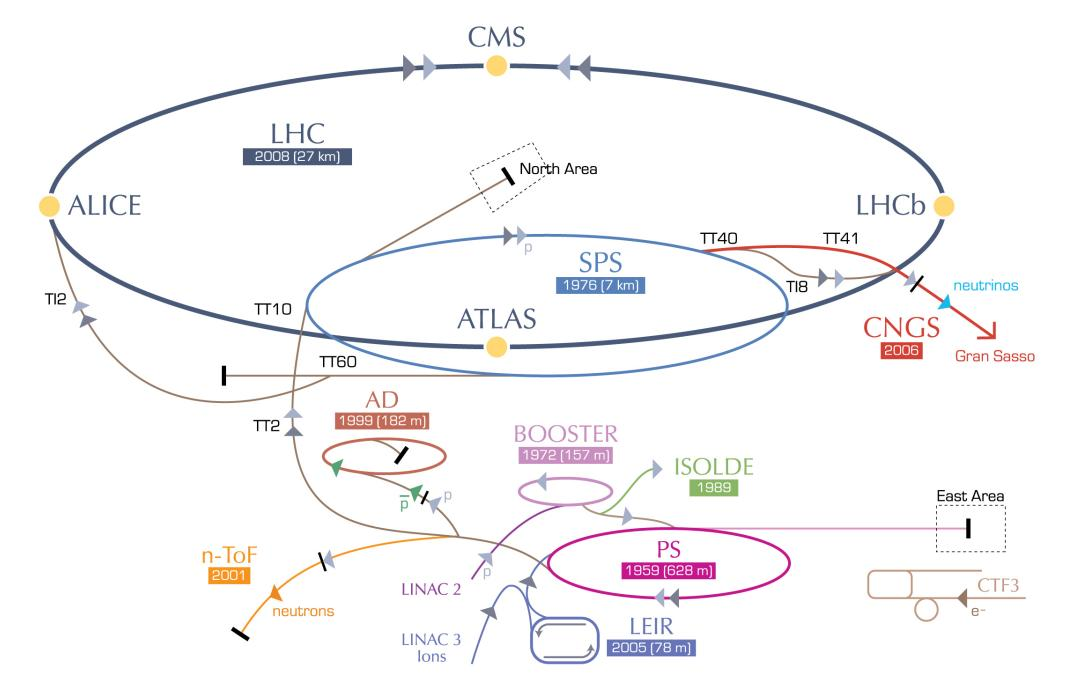
\includegraphics[scale=0.35]{LHC/CERNkomplex}
	\caption[Beschleunigerkomplex des CERN]{Beschleunigerkomplex des CERN, inklusive der vier gr\"o\"sten Experimente des LHC \cite{cernkomplex}.}
	\label{cernkomplex}
\end{figure}

% ======================
% ++++     LHC      ++++
% ======================
\subsection{Der Large Hadron Collider}
Der LHC ist mit einem Umfang von 26,7\,km der bislang größte von Menschen gebaute Teilchenbeschleuniger. Der Tunnel, bei dem Protonen zu einer Schwerpunktsenergie von bis zu 14\,TeV beschleunigt werden, liegt in 100\,m Tiefe am CERN\footnote{Europäische Organisation für Kernforschung. Formal \textbf{C}onseil \textbf{E}uropéen pour la \textbf{R}echerche \textbf{N}ucléaire.}-Gelände und dessen Umgebung.\\
Die durch Ionisation von Wasserstoff erzeugten Protonen \cite{duoplasma} durchlaufen eine Reihe von verschiedenen Vorbeschleunigern, bevor die Protonen in zwei gegenläufige Röhren des LHC injiziert werden \ref{cernkomplex}. 
Diese Vor\-be\-schleuniger\-reihe besteht aus einem Linearbeschleuniger (LINAC 2), dem Proton Synchrotron (PS) und dem Super Proton Synchrotron (SPS). Die Protonen werden am PS auf 25\,GeV und anschließend am SPS auf 450\,GeV beschleunigt, ehe sie in den LHC eingespeist und an vier festgelegten Punkten zur Kollision gebracht werden. Diese Kollisionspunkte sind von den folgenden Detektoren ummantelt:
\begin{itemize}
\item ALICE (A Large Ion Collider Experiment)
\item ATLAS (A Toroidal LHC Apparatus)
\item CMS (Compact Muon Solenoid)
\item LHCb (Large Hadron Collider beauty experiment)
\end{itemize}
Die Multifunktionsdetektoren ATLAS \cite{atlas} und CMS sind so konstruiert, dass eine Vielzahl von Standardmodell-Messungen und darüber hinaus Suchen nach Physik jenseits des Standardmodells möglich sind. Außerdem konnten die ATLAS- und CMS-Experimente bereits die Existenz des Higgs-Bosons nachweisen.\\
Im Gegensatz zu den Multifunktionsdetektoren sind ALICE \cite{alice} und LHCb \cite{lhcb} für speziellere Aufgaben konstruiert. So werden bei ALICE Blei-Ionen zur Kollision gebracht, um ein Quark-Gluon-Plasma zu erzeugen und zu untersuchen. Beim LHCb-Experiment wird die CP-Verletzung von B-Mesonen untersucht.
\\
Einer der großen Vorteile des LHC im Vergleich zu vorherigen Experimenten ist seine hohe Luminosität. Die Luminosität beschreibt die Anzahl der Teilchenbegegnungen pro Zeit und Fläche und ergibt sich aus
\begin{equation}
L=\frac{n_{b}N_{p}^{2}f}{A},
\end{equation}
wobei $n_{b}$ die Anzahl der B\"undel im Teilchenstrahl, $N_{p}$ die Anzahl der Protonen im B\"undel und $f$ die Umlauffrequenz der B\"undel ist. Die Gr\"o\ss{}e $A$ entspricht der effektiven Breite des Strahls in transversaler Richtung.\\
Als Designparameter f\"ur den LHC sind dabei $n_{b}=2808$ B\"undel mit $N_{p}=1,15\cdot 10^{11}$ Protonen pro B\"undel, eine Umlauffrequenz $f=11,25$\,kHz und dar\"uber hinaus eine Luminosit\"at von $L=10^{34}$cm$^{-2}$s$^{-1}$ vorgesehen. Als ein Ma\ss{} f\"ur die Gesamtzahl von Kollisionen und der damit gesammelten Gesamtdatenmenge wird die integrierte Luminosit\"at $L_{\rm{int}}=\int L dt$ eingef\"uhrt. In diesem Praktikumsversuch untersuchen Sie einen Datensatz mit einer integrierten Luminosit\"at von 50 pb$^{-1}$.
% Abbildung \ref{intlumi} zeigt die im Jahr 2012 aufgenommene integrierte Luminosit"at bei einer Schwerpunktsenergie von 8\,TeV. Der LHC lieferte 23,3\,fb$^{-1}$, wovon der CMS-Detektor 21,8\,fb$^{-1}$ aufgenommen hat \cite{lhclumi}.

\subsection{Teilchen-Identifizierung im Detektor}
Bei den Kollisionen der Protonen entstehen etliche neue Teilchen, die in alle Richtungen auseinander fliegen und mit Hilfe eines Detektors vermessen werden. In Kapitel \ref{kapsm} haben wir die Teilchen des Standard-Modells aufgelistet. Nicht alle diese Teilchen k\"onnen direkt im Detektor beobachtet werden. So zerfallen beispielsweise die Bosonen (W, Z und Higgs) viel zu schnell, sodass lediglich die Zerfallsprodukte beobachtet und vermessen werden k\"onnen. Identifizierbar sind z.B. Elektronen, Myonen sowie Photonen. Freie Quarks konnten bislang nicht beobachtet werden, jedoch werden sie als B\"undel von Teilchen, sogenannten Jets identifiziert.

Ein aus heutiger Sicht gew\"ohnlicher Detektor besteht aus mehreren Komponenten. Diese Komponenten sind in verschiedenen Lagen \textit{ziebelschalenf\"ormig} umeinander angeordnet. Der CMS-Detektor ist neben dem ATLAS-Detektor einer der beiden Multifunktionsdetektoren am LHC. Ein schematischer "Uberlick des CMS-Detektors mit den meisten seiner Komponenten ist Abbildung \ref{cmsdetektor} zu entnehmen. Die namensgebende Komponente ist der supraleitende Solenoid, welcher ein Magnetfeld von bis zu $B=4$\,T parallel zum Teilchenstrahl generiert. Die weiteren Komponenten werden im Folgenden beschrieben.\\

	\begin{figure}[t]
		\centering
		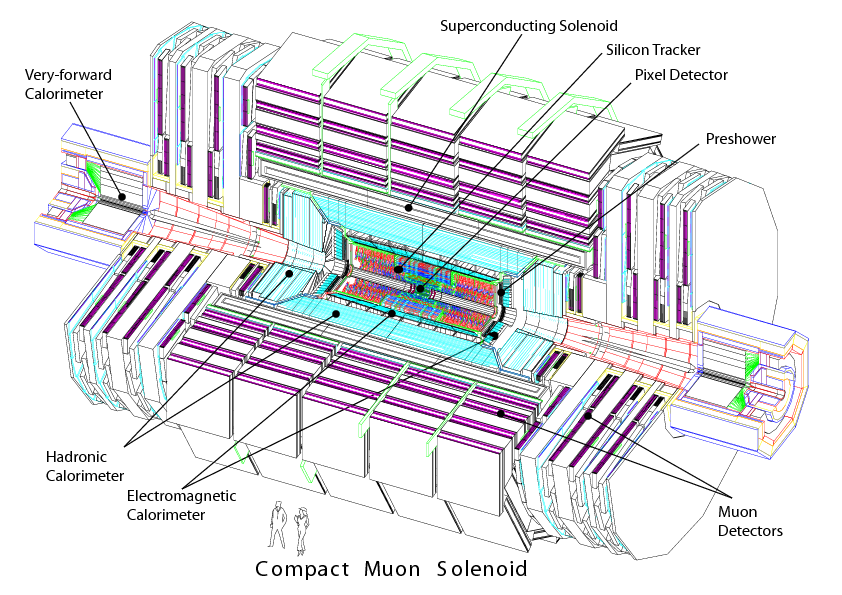
\includegraphics[scale=0.50]{LHC/cms_complete}
		\caption[Der CMS-Detektor]{Der CMS-Detektor \cite{Chatrchyan:2008aa}.}
		\label{cmsdetektor}
	\end{figure}

\begin{itemize}
\item \textbf{Spurdetektor}. Im inneren des CMS-Detektors befinden sich sogenannte Spurdetektoren aus Silizium, die die Messung von Ladung, Richtung und Impuls von geladenen Teilchen zur Aufgabe haben. Ausserdem wird der Entstehungsort der geladenen Teilchen bestimmt. Dies ist insbesondere von Bedeutung um Mesonen zu identifizieren. Das b-Quark bzw. b-Mesonen spielen dabei eine besondere Rolle, weil sie eine vergleichsweise lange Lebensdauer haben. Diese Mesonen legen aufgrund ihrer Lebensdauer im Mittel einen Weg von einigen Millimetern zur\"uck, ehe sie in leichtere Teilchen zerfallen und k\"onnen so von anderen Mesonen unterschieden werden. 
\item \textbf{Kalorimeter}. In den Kalorimetern des CMS-Detektors wird die Energie der entstandenen Teilchen bestimmt. Beim Zusammensto{\ss} der Teilchen mit Materie entstehen neue Teilchen und Photonen, dessen Energie anschlie{\ss}end vermessen wird.\\
Unterschieden wird dabei zwischen dem elektromagnetischen und dem hadronischen Kalorimeter. Das elektromagnetische Kalorimeter (bestehend aus 80.000 Bleiwolframat-Kristallen) misst die Energie von Elektronen und Photonen mit hoher Pr\"azision, indem diese Teilchen im Material einen elektromagnetischen Schauer erzeugen.\\
Das daran anschlie{\ss}ende hadronische Kalorimeter dient der Energiemessung der Hadronen, wie z.B. der Protonen oder Neutronen. Hier sind abwechselnd Lagen aus einem Material mit hoher Dichte (beim CMS-Detektor handelt es sich um Messing) als Absorbermaterial sowie Plastik-Szintillatoren als aktives Medium angebracht. 
\item \textbf{Myondetektor}. Die einzigen geladenen Teilchen, die in den Kalorimetern nicht absorbiert werden k\"onnen und diese durchdringen, sind Myonen. Zur Vermessung der Myonen ist der Magnet von sogenannten Myon-Kammern umgeben. Diese Kammern sind mit Gas gef\"ullt. Das Gas wird von den geladenen Myonen ionisiert und l\"osen so ein elektrisches Signal aus.
\end{itemize}

\subsection{Jets und Jet Energie Korrekturen} 
Als Jets bezeichnet man ein B"undel von Hadronen, welches in die Richtung des Ursprungs-Quarks fliegt (siehe Hadronisierung). Wie jedes experimentell rekonstruierte Objekt m\"ussen auch Jets kallibriert werden. Die von der CMS-Gruppe bestimmten Korrekturen der Jet Energieskala ber\"ucksichtigen zusätzliche Energiebeitr\"age aus weiteren Proton-Proton Kollisionen (Pile-up), die Response des Detektors und weitere Detektoreffekte. Diese Jet Energie Korrekturen (JEC) sind f\"ur viele Analysen von gro\ss{}er Bedeutung und zumeist eine der wichtigsten ssystematischen Unsicherheiten.  

% xyz kann rekonstruiert werden, zyx nicht. xyz kann rekonstruiert werden in folgenden Subdetektorkomponenten. Richtung und Impuls wird aus Tracker und Magnetfeld bestimmt, Energie aus Kalorimetern
%Zyx kann aus den beobachtbaren Teilchen rekonstruiert werden -> Bedingungen bla


% +++++++++++++++++++ Spurdetektor +++++++++++++++++++++++
%\subsubsection*{Spurdetektor}
%\label{kapinnertracking}
%Zur Messung der Ladung, der Richtung und des Impulses von geladenen Teilchen ist eine pr"azise Spurrekonstruktion notwendig. Der Spurdetektor ist die innerste Komponente des CMS-Detektors und zylindrisch aufgebaut. Seine sensiblen Bauteile sind auf Silizium basierende Sensoren, welche die durch Ionisation verloren gegangene Energie geladener Teilchen messen. 
%
%
%
%\subsubsection*{Elektromagnetisches Kalorimeter}
%\label{kapemkalo}
%Das elektromagnetische Kalorimeter (ECAL) umgibt den Spurdetektor und dient zur Messung der Energie von Elektronen und Photonen, die im Material einen elektromagnetischen Schauer erzeugen. Es ist beispielsweise von wesentlicher Bedeutung zur Identifizierung eines Higgs-Bosons im Zerfallskanal $H\rightarrow \gamma\gamma$. 
%\\
%Die Leistungsf"ahigkeit des ECALs wird mit Hilfe eines Teststrahls gemessen. Die Energieaufl"osung f"ur Elektronen als Funktion der Energie kann daher wie folgt parametrisiert werden \cite{Chatrchyan:2008aa}:
%\begin{equation}
%\left(\frac{\sigma(E)}{E}\right)^{2}=\left(\frac{a}{\sqrt{E/\text{GeV}}}\right)^{2}+\left(\frac{b}{E/\text{GeV}}\right)^{2}+\left(c\right)^{2}.
%\end{equation}
%Der erste Term wird aufgrund der elektromagnetischen Schauer eingef"uhrt und ist von statistischer Natur. Der zweite Term beschreibt das Rauschen der Elektronik. Der konstante Term ist beispielsweise auf Kalibrationsfehler oder das nichtlineare Ansprechverhalten zur"uckzuf"uhren.
%
%
%
%\subsubsection*{Hadronisches Kalorimeter}
%\label{kaphadkalo}
%Das hadronische Kalorimeter (HCAL) dient der Mess\-ung der Energie von geladenen und neutralen Hadronen. Da Hadronen bei gleicher Prim"ar\-energie tiefer in Material eindringen als Photonen und geladene Leptonen, liegt das HCAL au"serhalb des ECALs und umgibt es.\\
%
%
%
%\subsubsection*{Myon-System}
%\label{kapmyonsys}
%Die am weitesten au"sen liegende Komponente des CMS-Detektors ist das Myon-System. Das Myon-System wird ben"otigt, weil Myonen als minimal ionisierende Teilchen sowohl den Spurdetektor als auch die Kalorimeter ohne auff"allige Energieverluste durchqueren. Betrachtet man den Wechselwirkungspunkt als den Ursprung der Myonen, so ist die Bestimmung des Ablenkswinkels im Myon-System essentiell f"ur eine Messung des Impulses von Myonen.\\




%\subsubsection{Trigger und Datenerfassung}
%\label{trig}
%Die Kollisionsrate der Teilchenb"undel betr"agt am LHC 40\,MHz f"ur die Designluminosit"at. Diese Rate entspricht ungef"ahr 10$^{9}$ Wechselwirkungen pro Sekunde, wovon jedes Ereignis eine Datengr"o"se von 1\,MB hat. Es k"onnen jedoch lediglich einige hundert Wechselwirkungen pro Sekunde gespeichert werden. Der Trigger hat deshalb die Aufgabe, potentiell interessante Ereignisse schnell und effizient zu selektieren. Das Trigger-System arbeitet dabei in zwei Schritten.\\
%\\
%Zun"achst wird im Level-1(L1) Trigger die Rate von weiter zu prozessierenden Ereignissen auf maximal 100\,kHz reduziert. Dieses geschieht "uber eine vereinfachte Ereignisrekonstruktion, bei der einzig die Daten aus schnellen Detektorkomponenten, wie die Kalorimeter oder das Myon-System, ausgew"ahlt werden. Die Zeit f"ur eine Entscheidung ist im L1 Trigger auf 3,2\,$\mu$s pro Ereignis beschr"ankt. M"ogliche Teilchenkandidaten werden danach "uber vereinfachte Algorithmen rekonstruiert. Letzten Endes wird ein Ereignis auf Basis von festgelegten Grenzwerten, z.B. f"ur die transversale Energie $E_{T}$ oder den transversalen Impuls $p_{T}$ von Photonen, Elektronen, Myonen oder Jets, selektiert.\\
%\\
%Im zweiten Schritt k"onnen mit Hilfe des auf Software beruhenden High-Level-Triggers (HLT) Informationen aus allen Komponenten des Detektors mit h"oher entwickelten Algorithmen analysiert werden. Potentiell interessante Ereignisse werden auf Basis umfangreicher Eigenschaften selektiert, sodass eine Ereignisrate von n"aherungsweise 300\,Hz erreicht wird. Die Zeit f"ur eine Entscheidung des HLTs ist dabei auf 50\,ms pro Ereignis beschr"ankt.
%\\
%Um die finale Ereignisrate trotz ansteigender Luminosit"at auf dem Designwert zu halten, sind unterschiedliche Methoden m"oglich. Optimal w"aren verbesserte Algorithmen, die den Untergrund st"arker unterdr"uckt. Anderenfalls k"onnen die Trigger Grenzen erh"oht werden, wodurch jedoch die Effizienz des Signals verloren gehen kann. Des Weiteren be\-steht die M"oglichkeit eine zu hohe Triggerrate mit festgelegten Grenzen aufrecht zu erhalten, indem Ereignisse mit einem \textit{prescale} $n$ aufgenommen werden, sodass lediglich jedes $n$-te Ereignis erfasst wird.



\section{Datensatz und Monte-Carlo-Simulation}
\label{datasets}
Die Kollisionsrate der Protonen ist am LHC extrem hoch, sodass nicht alle Ereignisse gespeichert werden k\"onnen. Ein Trigger-System selektiert deshalb interessante Ereignisse und reduziert damit die totale Rate an Ereignissen. Der Trigger, der f\"ur diese Analyse benutzt wurde selektiert Ereignisse, die isolierte Myonen mit einem Transversalimpuls von $p_{T}>24$ GeV beinhalten. Das Sample mit echten Daten, die mit dem CMS-Detektor und dem Trigger aufgenommen wurden, hat 469384 Ereignisse. Dieses entspricht einer integrierten Luminosit\"at von 50 pb$^{-1}$. Weitere Details sind in Tabelle \ref{table_samples} zu finden.\\
Diese Tabelle beinhaltet dar\"uber hinaus Informationen \"uber die simulierten Samples. Die Anzahl der simulierten Ereignisse kann erheblich kleiner oder gr\"o\ss{}er sein als f\"ur 50 pb$^{-1}$ ben\"otigt, da die Ereignisse aus Simulationen entsprechend gewichtet werden k\"onnen. Dieses Gewicht ist als \textbf{EventWeight} - Variable in jedem simulierten Sample gespeichert. Damit die simulierten Samples jeweils einer integrierten Luminosit\"at von 50 pb$^{-1}$ entsprechen, m\"ussen alle Ereignisse mit ihrem \textbf{EventWeight} gewichtet (''multipliziert'') werden.
\begin{small}
\begin{table}[h!]
  \centering
  \begin{tabular}{|l|c|c|c|}
    \hline 
Datei-Name & Prozess & $\#$Ereignisse & WQS \\ \hline\hline
data.root & Daten & 469384 & \\ \hline
ttbar.root & sim. $t\bar{t}$-Signal & 36941 & 165 pb  \\
wjets.root & sim. W+Jets Untergrund & 109737 & 31300 pb \\
dy.root & sim. Drell-Yan Untergrund & 77729 & 15800 pb \\
ww.root & sim. WW Untergrund & 4580 & 43 pb \\
wz.root & sim. WZ Untergrund & 3367 & 18 pb \\
zz.root & sim. ZZ Untergrund & 2421 & 6 pb \\
single\_top.root & sim. Single Top Untergrund & 5684 & 85 pb \\
qcd.root & sim. QCD Multijet Untegrund & 142 & $10^8$ pb \\
    \hline
  \end{tabular}
  \caption{Daten und simulierte MC-Samples.}
  \label{table_samples}
\end{table}
\end{small}
\\Wie Sie des Weiteren der Tabelle entnehmen k\"onnen, enth\"alt das QCD-Multijet-Sample nur noch sehr wenige getriggerte Ereignisse, obwohl der Produktions-Wirkungsquerschnitt f\"ur diesen Prozess sehr gro\ss{} ist. Dieser Untergrund wird bereits aufgrund des Triggers stark reduziert, da dort ein isoliertes Myons verlangt wird.\\
Alle (ROOT-)Dateien sind in Unterordnern des HEPTutorial.tar.gz - Pakets zu finden.

%\section{Datenformat und Struktur des ROOT tree}
\label{dataformat}
Die in Kapitel \ref{datasets} beschriebenen Samples sind in sogenannten \texttt{ROOT trees} gespeichert. Diese \texttt{trees} beinhalten eine Kollektion von Variablen, die pro Ereignis gef\"ullt sind. Die Liste der Variablen inklusive ihres Datentyps ist im Folgenden gegeben. Variablen mit Klammern \texttt{[]} bedeuten, dass sie als \texttt{Array} gespeichert sind.
\begin{itemize}
	\item \texttt{NJet} (integer): Anzahl von Jets im Ereignis.
	\item \texttt{Jet\_Px[NJet]} (float): x-Komponente von Jet-Impulsen. Es handelt sich hierbei um ein Array der Gr\"o\ss{}e \texttt{NJet}, wobei maximal 20 Jets gespeichert werden. Sofern es mehr als 20 Jets in einem Ereignis gibt, werden nur die 20 Jets mit der gr\"o\ss{}ten Energie gespeichert. Des weiteren werden ausschlie\ss{}lich Jets mit $p_{T}>30$ GeV gespeichert.
	\item \texttt{Jet\_Py[NJet]} (float): y-Komponente von Jet-Impulsen.
	\item \texttt{Jet\_Pz[NJet]} (float): z-Komponente von Jet-Impulsen.
	\item \texttt{Jet\_E[NJet]} (float): Energie des Jets. Hinweis: die Komponenten \texttt{Jet\_Px[NJet]}, \texttt{Jet\_Py[NJet]}, \texttt{Jet\_Pz[NJet]} und \texttt{Jet\_E[NJet]} bilden den Vierervektor des Jets und beschreiben damit vollst\"andig die Kinematik eines Jets.
	\item \texttt{Jet\_btag[NJet]} (float): b-tagging Diskriminator. Diese Gr\"o\ss{}e erh\"alt man aus einem Algorithmus, welcher Zerf\"alle von B-Hadronen identifiziert. Gr\"o\ss{}ere Werte weisen auf eine h\"ohere Wahrscheinlichkeit hin, dass das Jet aus einem b-Quark stammt.
	\item \texttt{Jet\_ID[NJet]} (bool): dient zur Unterscheidung von echten Jets (aus hadronischen Wechselwirkungen) und Detektor-St\"orsignalen. Ein $guter$ Jet hat \texttt{true} als Wert.
	\item \texttt{NMuon} (integer): Anzahl der Myonen im Ereignis.
	\item \texttt{Muon\_Px[NMuon]} (float): x-Komponente von Myon-Impulsen.
	\item \texttt{Muon\_Py[NMuon]} (float): y-Komponente von Myon-Impulsen.
	\item \texttt{Muon\_Pz[NMuon]} (float): z-Komponente von Myon-Impulsen.
	\item \texttt{Muon\_E} (float): Energie des Myons.
	\item \texttt{Muon\_Charge} (integer): Ladung des Myons. Diese wird aus der Kr\"ummung im Magnetfeld bestimmt und hat die Werte +1 oder -1.
	\item \texttt{Muon\_Iso[NMuon]} (float): Myon-Isolation. Diese Variable ist ein Ma\ss{} f\"ur die Menge an Detektor-Aktivit\"at in der N\"ahe des Myons. So haben z.B. Myonen innerhalb von Jets einen gro\ss{}en Wert f\"ur \texttt{Muon\_Iso}. Myonen, die aus W-Zerf\"allen stammen, haben typischerweise kleine Werte f\"ur \texttt{Muon\_Iso}.
	\item \texttt{NElectron} (integer): s. Beschreibung der Myonen
	\item \texttt{Electron\_Px[NElectron]} (float): s. Beschreibung der Myonen
	\item \texttt{Electron\_Py[NElectron]} (float): s. Beschreibung der Myonen
	\item \texttt{Electron\_Pz[NElectron]} (float): s. Beschreibung der Myonen
	\item \texttt{Electron\_E} (float): s. Beschreibung der Myonen
	\item \texttt{Electron\_Charge} (integer): s. Beschreibung der Myonen
	\item \texttt{Electron\_Iso[NElectron]} (float): s. Beschreibung der Myonen
	\item \texttt{NPhoton} (integer): s. Beschreibung der Myonen
	\item \texttt{Photon\_Px[NPhoton]} (float): s. Beschreibung der Myonen
	\item \texttt{Photon\_Py[NPhoton]} (float): s. Beschreibung der Myonen
	\item \texttt{Photon\_Pz[NPhoton]} (float): s. Beschreibung der Myonen
	\item \texttt{Photon\_E} (float): s. Beschreibung der Myonen
	\item \texttt{Photon\_Iso[NPhoton]} (float): s. Beschreibung der Myonen
	\item \texttt{MET\_px} (float): x-Komponente der fehlenden transversalen Energie. Objekte wie Neutrinos, die den Detektor entgehen, verursachen fehlende transversale Energie, welche gemessen und mit dem Neutrino assoziiert werden kann.
	\item \texttt{MET\_py} (float): y-Komponente der fehlenden transversalen Energie.
	\item \texttt{NPrimaryVertices} (integer): Anzahl der Vertizes von Proton-Proton-Interaktionen. Aufgrund der hohen Luminosit\"at am LHC k\"onnen mehrere Protonen innerhalb eines Teilchenb\"undels kollidieren. Dieses wird typischerweise als \texttt{pile-up} bezeichnet.
	\item \texttt{triggerIsoMu24} (bool): Trigger \texttt{bit}. Sofern ein Ereignis getriggert wurde ist dieser Wert \texttt{true}, andernfalls \texttt{false}. 
\end{itemize}
Alle oben beschriebenen Gr\"o\ss{}en werden mit dem Detektor gemessen und sind sowohl f\"ur echte Daten als auch f\"ur Monte-Carlo-Simulationen verf\"ugbar. 


\section{Analyse-Framework}
\label{framework}
Das Paket TopWQS.tar.gz enth\"alt eine (unvollst\"andige) Analyse-Software, auf dessen Basis Sie Ihre Versuchsdurchf\"uhrung beginnen werden. Eine Beschreibung der individuellen Komponenten der Analyse-Software ist in der folgenden Liste zu finden. Dort sind ebenso Hinweise, wie Sie beginnen sollten den Code zu erweitern.
\begin{itemize}
	\item \textbf{example.C}: Diese Datei ist ihr Startpunkt. Es beinhaltet die \texttt{main()} Funktion, welche f\"ur jedes C\texttt{++} Programm unabdingbar ist. Dar\"uber hinaus finden Sie hier Instanzen aus \texttt{MyAnalysis}, die in den Dateien \texttt{MyAnalysis.h} und \texttt{MyAnalysis.C} implementiert sind. Das \texttt{TChain} repr\"asentiert den \texttt{ROOT tree} (s. Kapitel \ref{dataformat}). Die Dateien, die gelesen werden, sind in der Funktion \texttt{Add(filename)} spezifiziert. Der \texttt{tree} wird mit der \texttt{Process()} Funktion gelesen und prozessiert, indem es ein Argument aus \texttt{MyAnalysis} benutzt. Folglich findet der Gro\ss{}teil Ihrer Arbeit in der \texttt{Process()} Funktion aus der \texttt{MyAnalysis} Klasse statt.
	\item \textbf{MyAnalysis.h}: Definition der Klasse \texttt{MyAnalysis}, welcher aus \texttt{ROOT TSelector} erbt. Der Konstruktor verwendet einen globalen Skalierungsfaktor (welcher standardm\"a\ss{}ig auf 1,0 gesetzt ist), der auf alle Ereignisse in den jeweiligen Samples angewendet wird. Dieser Skalierungsfaktor wird benutzt um die MC-Prozesse (ent\-sprech\-end der Anzahl der simulierten Ereignisse und ihres Wirkungsquerschnitts) zu normieren. \texttt{MyAnalysis} beinhaltet die Deklaration aller Variablen, die im ROOT tree gespeichert sind. Dar\"uber hinaus werden hier Variablen und Funktionen deklariert, die Sie in Ihrer Analyse benutzen werden (z.B. deklarieren Sie hier Ihre Histogramme). 
	\item \textbf{MyAnalysis.C}: die beiden main-Funktionen, die automatisch aufgerufen werden w\"ahrend der ROOT tree prozessiert wird, sind \texttt{SlaveBegin()} und \texttt{Process()}. Die \texttt{SlaveBegin()} Funktion wird einmal pro Job aufgerufen, direkt bevor die Ereignisse prozessiert werden. Es dient dazu Histogramme einzutragen. Die \texttt{Process()} Funktion wird automatisch f\"ur jedes einzelne Ereignis aufgerufen. Hier ist der Kern der Analyse implementiert. 
	\item \textbf{MyMuon.h/MyMuon.C}: erbt von \texttt{TLorentzVector}, was grunds\"atzlich einem Vierervektor entspricht. Dar\"uber hinaus werden zus\"atzliche Informationen, wie die Ladung und Isolation des Myons dem Vierervektor hinzugef\"ugt.
	\item \textbf{MyElectron.h/MyElectron.C}: s. \texttt{MyMuon}, entsprechend f\"ur Elektronen.
	\item \textbf{MyJet.h/MyJet.C}: erbt von \texttt{TLorentzVector} und addiert Informationen zum Vierervektor \"uber die b-tagging-Variable. Die b-tagging-Variable is korreliert mit der Wahrscheinlichkeit, dass das Jet aus einem b-Quark stammt. Gro\ss{}e Werte dieser Variable sind gleichbedeutend mit einer gro\ss{}en Wahrscheinlichkeit, dass es sich um ein b-Quark-Jet handelt. Die Funktion \texttt{IsBTagged()} schneidet auf den b-tag Diskriminator und gibt einen \texttt{boolean} wieder (\texttt{true} oder \texttt{false}). Die Funktion \texttt{GetJetID()} gibt \texttt{true} wieder, sofern ein Jet ausreichend Kriterien erf\"ullt, andernfalls wird \texttt{false} wieder gegeben.
	\item \textbf{Plotter.h/Plotter.C}: Mit diesem Tool k\"onnen mehrere Histogramme, die als \texttt{std::vector} gespeichert sind, graphisch dargestellt werden.
\end{itemize}


\newpage
\section{Vorbereitung (vor Praktikumsbeginn)}
%\section{Durchf\"uhrung}
\label{tasks}
Wie \"ublich beginnt auch dieser Praktikumsversuch mit einer Vorbesprechung, in der zun\"achst der theoretische Hintergrund der Analyse diskutiert wird. Im Folgenden finden Sie einen Fragenkatalog, der Ihnen einen Eindruck des Erwartungshorizonts vermittelt.\\
\underline{Physik des Top-Quarks}
\begin{itemize}
	\item Wann und wo wurde das Top-Quark entdeckt?
	\item Wie schwer ist das Top-Quark? Wie schwer ist es verglichen mit den anderen Teilchen des Standard-Modells?
	\item Wie werden Top-Quarks (sowohl einzeln als auch in Paaren) am Large-Hadron-Collider erzeugt?
	\item Wie zerfallen Top-Quarks? Was versteht man unter dem voll-hadronischen, semi-leptonischen und dileptonischen Zerfallskanal?
	\item Welche Zerfallsprodukte des Top-Quarks k\"onnen mit einem Detektor tats\"achlich gemessen werden?
	\item Welche anderen (Untergrund)Prozesse ergeben im Detektor wom\"oglich dieselbe Signatur wie ein $t\bar{t}$-Ereignis?
	%\item wie berechnet man den inklusiven Wirkungsquerschnitt f\"ur $t\bar{t}$-Produktion?
\end{itemize}
\underline{Detektor-Physik}
\begin{itemize}
	\item Wie misst man den Impuls eines geladenen Teilchens?
	\item Wie wird die Energie von Elektronen und Photonen gemessen?
	\item Wie wird die Energie von Hadronen gemessen?
	\item Warum wird ein separates Myon-System ben\"otigt? Wie funktioniert es?
\end{itemize}
\underline{Wichtige Gr\"o\ss{}en an modernen Collidern}
\begin{itemize}
	\item Was ist (integrierte) Luminosit\"at? Wie ist sie definiert?
	\item Was versteht man unter dem Transversalimpuls $p_{T}$?
	\item Was ist die Pseudorapidit\"at $\eta$ definiert? Warum wird diese Gr\"o\ss{}e gegen\"uber dem Polarwinkel $\theta$ bevorzugt?
	\item Was versteht man unter fehlender transversaler Energie und woher kommt sie?
	\item Was versteht man unter dem sogenannten b-tagging?
\end{itemize}


\section{Aufgaben}
F\"ur die Durchf\"uhrung des Versuchs wird Ihnen ein Unix-Rechner zur Verf\"ugung gestellt. Sie loggen sich auf einem Gast-Konto ein. Die ben\"otigte Software befindet sich bereits auf dem Rechner. \"Offnen Sie eine Konsole und erstellen Sie sich einen Ordner, z.B.:
\begin{lstlisting}
mkdir mydir
cd mydir
\end{lstlisting}
In diesem Ordner f\"uhren Sie den Versuch durch und speichern alle Ergebnisse.
%Hinweis: Sie loggen sich mit einem Gast-Konto ein. Bringen Sie bitte au\ss{}erdem f\"ur Ihre Auswertung einen USB-Stick mit, um Ihre Ergebnisse zu sichern. Die zur Verf\"ugung gestellten Rechner arbeiten im Offline-Betrieb.
\subsection{Event Displays mit der Fireworks-Software}
Die Fireworks-Software wird zur graphischen Darstellung von Ereignissen im Detektor verwendet. Kopieren Sie sich die Software wie folgt in Ihren Ordner:
\begin{lstlisting}
cp -r /opt/fp/cmsShow-8.1 .
cp -r /opt/fp/sources .
\end{lstlisting}
Sie betrachten im Folgenden ein Sample mit 400 simulierten $t\bar{t}$-Ereignissen. \"Offnen Sie das $t\bar{t}$-Sample wie folgt:
\begin{lstlisting}
cd cmsShow-8.1
./cmsShow ../sources/ttbar.root
\end{lstlisting}
Machen Sie sich nun mit der Software vertraut:
\begin{itemize}
\item betrachten Sie verschiedene Ereignisse
\item machen Sie sich klar, welche Anzeigen welche Objekte darstellen
\item betrachten Sie Ereignisse in der Rho-Z-Achse sowie im 3D-Tower.
\end{itemize}
Versuchen Sie nun jeweils ein Ereignis f\"ur den voll-hadronischen, semi-leptonen und di-leptonen Zerfallskanal zu klassifizieren. Benutzen Sie daraufhin die Filter-Funktion. Passen Sie diese so an, dass m\"oglichst ausschlie{\ss}lich $t\bar{t}$-Ereignisse im semi-leptonischen Zerfallskanal betrachtet werden. Speichern Sie (mindestens) ein Event-Display f\"ur Ihre Auswertung!\\
\\
Betrachten Sie nun Event-Displays aus einem Single-Top-Sample:
\begin{lstlisting}
./cmsShow ../sources/singletop.root
\end{lstlisting}
K\"onnen Sie Unterschiede feststellen, die Ihnen bei der Selektion von $t\bar{t}$-Ereignissen helfen? Speichern Sie f\"ur Ihre Auswertung ein Event-Display mit einem Single-Top-Ereignis.

\subsection{Einf\"uhrung in das Analyse-Framework}
Unser Analyse-Framework ist bereits voll funktionsf\"ahig, jedoch macht es bislang nicht viel. Setzen Sie das Analyse-Framework auf und f\"uhren Sie es ein erstes Mal aus:
\begin{itemize}
	%\item erstellen Sie zun\"achst im Home-Verzeichnis einen neuen Ordner
	\item entpacken Sie dazu das Paket TopWQS.tar.gz mit 'tar -xf sources/TopWQS.tar.gz' in Ihren Ordner
	\item kompilieren Sie mit 'make'. Das Kompilieren erstellt Ihnen eine ausf\"uhrbare Datei \textbf{example.x}
	\item nun kann das Framework ausgef\"uhrt werden mit './example.x'
\end{itemize}
Das Programm schreibt bereits Output-Dateien (wie z.B. \textbf{nocuts.pdf}), die zwei Verteilungen der Analyse beinhalten. \"Offnen Sie die Dateien mit einem PDF-Viewer, wie z.B. \textbf{xpdf/okular}. Im Folgenden arbeiten Sie haupts\"achlich in den Dateien 'MyAnalysis.C', 'MyAnalysis.h' und 'example.C'. \"Offnen Sie diese mit einem Editor, z.B. Emacs, mit 'emacs MyAnalysis.C'. Machen Sie sich zu Beginn mit dem Code vertraut.

\subsection{Aufgabe 1: Eigenschaften von Top-Quark-Ereignissen}
In der Datei \textbf{nocuts.pdf} finden Sie verschiedene Verteilungen, wie z.B. die Anzahl der Myonen, Muon $p_{T}$, Anzahl der Jets, etc. in einem Ereignis. \\
\subsubsection{Aufgabe 1.1:}
\begin{itemize}
  \item Betrachten Sie die bereitgestellten Histogramme und machen Sie sich mit ihnen vertraut.
  \item Finden Sie heraus, wie viele Ereignisse in den Daten mehr als ein isoliertes und rekonstruiertes Myon haben. Aus welchen Prozessen stammen diese zus\"atzlichen Myonen? Betrachten Sie dazu die jeweiligen Monte-Carlo-Samples.
\end{itemize}
\subsubsection{Aufgabe 1.2}
In diesem Aufgabenteil beginnen wir mit den ersten Schritten hinsichtlich einer realen Messung mit Top-Quark-Ereignissen. Dazu m\"ussen wir verstehen, wie man Top-Quark-Ereignisse effizient selektiert und gleichzeitig den Anteil von Ereignissen ohne Top-Quarks (sogenannte Untergrund-Ereignisse) reduziert.
\begin{itemize}
        \item Fordern Sie von nun an f\"ur alle Verteilungen mindestens ein isoliertes Myon.
	\item Versuchen Sie Variablen zu finden, die besonders sensitiv sind um zwischen Signal und Untergrund zu unterscheiden. Geeignete Variablen k\"onnten z.B. die Anzahl von Jets, der Transversalimpuls des 1., 2., 3. Jets, der Transversalimpuls von Myonen, fehlende transversale Energie, die Anzahl von b-Jets (b-tagging), der Transversalimpuls des 1., 2. b-Jets sowie Winkelverteilungen ($\eta$) von (b-)Jets und Myonen sein. \\
	 Vergleichen Sie daf\"ur in den Histogrammen Signal mit Untergrund!
	\item Wenden Sie Schnitte auf verschiedene Variablen an um das Verh\"altnis aus Signal zu Untergrund zu verbessern. Wie viele Signal-Ereignisse verlieren Sie durch die Anwendung ihrer Selektion (Signal-Effizienz) und wie viele Ereignisse aus Untergrund-Prozessen? Welcher Untergrund ist besonders unangenehm? Lassen Sie sich sowohl die Effizienzen, als auch die Reinheit nach jedem Schnitt anzeigen. (Hinweis: f\"ugen Sie eine Variable, z.B. einen \textbf{float}, ein, die der Anzahl ihrer selektierten Ereignisse entspricht. Addieren Sie dazu das \textbf{Event\-Weight} auf Ihre eingef\"uhrte Variable nach der vollen Selektion f\"ur jedes Ereignis mit dem \grqq{}+=\grqq{} Operator.)
        \item Es empfiehlt sich iterativ vorzugehen, d.h. Sie wenden z.B. einen Schnitt auf mindestens 2 Jets an und \"uberpr\"ufen, was dieser Schnitt f\"ur Folgen hat, indem Sie sich wieder alle Verteilungen, sowie Reinheit und Effizienz ansehen. Dann wenden Sie sich der n\"achsten Variable (bzw. dem n\"achsten Schnitt) zu und verfahren genauso. Speichern Sie die Histogramme vor und nach den Schnitten. \\
\end{itemize}

\subsubsection{Aufgabe 2: Messung des Wirkungsquerschnitts}
Ziel dieser Aufgabe ist die Berechnung des Wirkungsquerschnitts der Top-Antitop-Quark-Produktion am LHC. Die ben\"otigten Gr\"o\ss{}en bestimmen Sie dazu Schritt f\"ur Schritt:
\begin{itemize}
	\item F\"ur die Berechung des Wirkungsquerschnitts ben\"otigen Sie die Akzeptanz(Signaleffizienz) $\epsilon$. Die Akzeptanz beinhaltet die Tatsache, dass wir uns auf den semileptonischen Zerfalls\-kanal mit einem Myon im Endzustand beschr\"anken. Dieses Verzweigungsverh"altnis ist bekannt und kann aus der Simulation genommen werden. Dar\"uber hinaus beinhaltet die Akzeptanz alle Selektions-Schnitte, die Sie in Aufgabe 2 eingef\"uhrt haben. \\Sie berechnen die Akzeptanz aus dem Verh\"altnis der Anzahl selektierter Top-Quark-Ereignisse (nach allen Schnitten) und der Anzahl aller generierten Top-Quark-Er\-eig\-nisse.
	\item Der Wirkungsquerschnitt wird mit Hilfe echter Daten berechnet. Allerdings beinhalten die Daten, auch nach Anwendung Ihrer Selektion, noch Untergrund-Ereignisse, die zur Berechnung des Wirkungsquerschnitts nicht mitgez\"ahlt werden d\"urfen. Wir vertrauen der Simulation insofern, dass sie die korrekte Anzahl von Untergrund-Ereignissen nach der Selektion vorhersagt. Bestimmen Sie die Anzahl an Top-Antitop-Quark-Ereignissen in den Daten, indem Sie die erwartete Anzahl von Untergrund-Ereignissen von den Daten-Ereignissen subtrahieren.
	\item Nun k\"onnen Sie den Wirkungsquerschnitt mit folgender Formel bestimmen: $\sigma_{t\bar{t}} = \frac{N^{data} - N^{bg}}{\epsilon \cdot L}$. Geben Sie einen Fehler auf Ihre Messung an! (Hinweis: Nehmen Sie f\"ur die Luminosit\"at einen Fehler von 5\% an)
        \item Durch die Anwendung von Jet Energie Korrekturen (JEC) ist es zudem notwendig, einen systematischen Fehler zu bestimmen. Wiederholen Sie dazu die Berechnung des Wirkungsquerschnitts und variieren Sie dabei die Jet Energie Korrekturen (up/down). 
	\item Vergleichen Sie ihr Resultat mit einem offiziellen Ergebnis von ATLAS oder CMS (z.B. http://arxiv.org/pdf/1108.3773.pdf)
\end{itemize}



\newpage
\section{Auswertung}
\label{prot}
Allgemeiner Hinweis: Achten Sie bitte auf sinnvolle Bild- und Tabellenbeschriftungen und f\"ugen Sie, wenn notwendig, Quellenangaben hinzu. Wir empfehlen einf\"uhrende Kapitel (wie das Theorie- und Detektor-Kapitel) bereits vor Praktikumsbeginn zu schreiben.\\
\\
Ihr Protokoll sollte den folgenden Inhalt umfassen:
\begin{enumerate}
	\item Einleitung
	\item kurze Einf\"uhrung in das Standard-Modell und insbesondere in die Physik des Top-Quarks
	\item kurze Einf\"uhrung zum Large-Hadron-Collider sowie den Komponenten des CMS-Detektors (max. 3 Seiten)
	\item Auswertung der Aufgaben
	\begin{itemize}
		\item Charakterisierung von Top-Antitop-Ereignissen (inkl. Event-Displays)
		\item Auflistung und Erl\"auterung Ihrer Schnitte (inkl. der von Ihnen erstellen Graphiken, vor und nach den Schnitten)
		\item Ergebnis f\"ur $\sigma_{t\bar{t}}$, inklusive Fehlerrechnung und einem Vergleich mit einem offiziellen Ergebnis von CMS und/oder ATLAS
                \item Rekonstruktion des $t\overline{t}$-Systems und Bestimmung der Masse
                \item Diskussion des Versuches/Verbesserungen 
       \end{itemize}
	\item Zusammenfassung / Fazit
\end{enumerate}

\bibliography{references}{}
\bibliographystyle{unsrt}

\end{document}